\documentclass[10pt,a4paper]{article}
\usepackage{amsmath,amssymb,amsthm,graphicx}
\usepackage{amsmath,amssymb,amsthm,graphicx,xcolor,mathrsfs,mathtools,tikz-cd}
\usepackage[shortlabels]{enumitem}
\setlist[enumerate,1]{label={\rm(\roman*)},ref={\rm\roman*}}
\usepackage[a4paper,margin=25mm]{geometry}
\usepackage[colorlinks=true,linkcolor=blue,citecolor=blue,urlcolor=blue]{hyperref}
\graphicspath{{items/}}
\emergencystretch=3em
\numberwithin{equation}{section}
\newcommand{\doi}[1]{\href{https://doi.org/#1}{doi:\nolinkurl{#1}}}
\newcommand{\arXiv}[1]{\href{https://arxiv.org/abs/#1}{arXiv:\nolinkurl{#1}}}
\providecommand{\bysame}{\leavevmode\hbox to3em{\hrulefill}\thinspace}
%%%%%%%%%%%%%%%%%%%%%%%%%%%%%%%%%%%%%

\theoremstyle{definition}
\newtheorem{definition}{Definition}[section]

\theoremstyle{plain}
\newtheorem{proposition}[definition]{Proposition}
\newtheorem{theorem}[definition]{Theorem}
\newtheorem{corollary}[definition]{Corollary}
\newtheorem{lemma}[definition]{Lemma}
\newtheorem{conjecture}{Conjecture}


\theoremstyle{remark}
\newtheorem{remark}[definition]{Remark}
\newtheorem{example}[definition]{Example}

\newtheorem{innercustomclaim}{Claim}
\newenvironment{claim}[1]{\renewcommand\theinnercustomclaim{#1}\innercustomclaim}{\endinnercustomclaim}

%%%%%%%%%%%%%%%%%%%%%%%%%%%%%%%%%%%%%
% Define any new command you need
%%%%%%%%%%%%%%%%%%%%%%%%%%%%%%%%%%%%%

\newcommand{\R}{\mathbb{R}}
\newcommand{\Z}{\mathbb{Z}}
\newcommand{\C}{\mathbb{C}}
\newcommand{\Q}{\mathbb{Q}}

\newcommand{\clin}{\mathbb{C}P^1}
\newcommand{\cp}{\mathbb{C}P^2}
\newcommand{\ppp}{\mathbb{C}P^1\times \mathbb{C}P^1\times \mathbb{C}P^1}
\newcommand{\cpp}{\mathbb{C}P^3}
\newcommand{\cpcp}{\mathbb{C}P^3\sharp\overline{\mathbb{C}P^3}}
\newcommand{\pp}{\mathbb{C}P^1\times \mathbb{C}P^1}

\newcommand{\rlin}{\mathbb{R}P^1}
\newcommand{\rplan}{\mathbb{R}P^2}
\newcommand{\rprp}{\mathbb{R}P^1\times \mathbb{R}P^1}
\newcommand{\rprprp}{\mathbb{R}P^1\times \mathbb{R}P^1\times \mathbb{R}P^1}
\newcommand{\ssrp}{\mathbb{S}^2\times \mathbb{R}P^1}
\newcommand{\rppp}{\mathbb{R}P^3}
\newcommand{\rprpsharp}{\mathbb{R}P^1\times \mathbb{R}P^1\sharp\overline{\mathbb{R}P^2}}
\newcommand{\rprpssharp}{\mathbb{R}P^1\times \mathbb{R}P^1\sharp 2\overline{\mathbb{R}P^2}}
\newcommand{\ssharp}{\mathbb{S}^2\sharp 2\overline{\mathbb{R}P^2}}

\DeclareMathOperator{\Crit}{Crit}
\DeclareMathOperator{\GW}{GW}
\DeclareMathOperator{\ind}{ind}
\DeclareMathOperator{\Pic}{Pic}
\DeclareMathOperator{\Sing}{Sing}
\DeclareMathOperator{\SO}{SO}
\DeclareMathOperator{\Pin}{Pin}
\DeclareMathOperator{\Spin}{Spin}
\DeclareMathOperator{\rank}{rank}
\DeclareMathOperator{\ev}{ev}
% query set upright
\renewcommand{\Im}{\operatorname{Im}}
\renewcommand{\sp}{\operatorname{sp}}
\newcommand{\Sym}{\operatorname{Sym}}
\newcommand{\PD}{\operatorname{PD}}
\newcommand{\pt}{\mathrm{pt}}

\newcommand{\sing}{\mathrm{sing}}
\renewcommand\labelitemi{$\bullet$}
\newcommand{\lra}{\longrightarrow}

\def\lowcong{\vbox to 0pt{\vss\hbox{$\scriptstyle\cong$}\vskip-1.5pt}}

\newcommand{\supth}[1]{\ensuremath{#1^{\mathrm{th}}}}
\usepackage{cleveref}
\crefname{originaltheorem}{original theorem}{original theorems}
\Crefname{originaltheorem}{Original theorem}{Original theorems}
\makeatletter
\newlabel{Theorem2-W}{{1.4}{source}{}{sourcepointer-1}{}}
\newlabel{Theorem2-W@cref}{{[originaltheorem][0][]1.4}{[1][0][]source}{}{}{}}
\makeatother
\crefname{originalcorollary}{original corollary}{original corollarys}
\Crefname{originalcorollary}{Original corollary}{Original corollarys}
\makeatletter
\newlabel{coro-degree.case.real}{{2.18}{source}{}{sourcepointer-2}{}}
\newlabel{coro-degree.case.real@cref}{{[originalcorollary][0][]2.18}{[1][0][]source}{}{}{}}
\makeatother
\title{Genus-zero del Pezzo threefold/surface Gromov-Witten correspondence (Theorem 1.3)}
\author{Thi Ngoc Anh Nguyen}
\date{arxiv:2302.09412; CC BY-SA 4.0}
\begin{document}
\maketitle
\noindent\textit{Allowed standard prerequisites (editorial).}\begin{itemize}
\item Del Pezzo classification, Bertini, adjunction and Riemann–Roch. [IP10], [Isk77], [Sho80], [GH78], [DPT09]; original Sections 1–2. External classification and standard surface/threefold geometry; current pencil degree argument is included.
\item Picard–Lefschetz and elliptic Picard geometry. [Ngu22], Section 2.2.2; classical Picard–Lefschetz formula and elliptic torsion count. External background; current rank-one monodromy and degree constructions retained.
\item Stable maps, enumerativity and balanced regularity. [KM94], [Vak97], [Cos09], [Wel05a] Proposition 2.2, [BG16] Section 5, [GH83] Theorem (4.f.3). External moduli/deformation tools; entire current Section 3 including the author’s two-claim nonsplitting/variation argument retained. No independent reproof of cited standard sources.
\end{itemize}\medskip
\ifdefined\hypertarget\hypertarget{sourcepointer-1}{}\fi
\noindent\textit{Source reference.} Original theorem 1.4: persistence-modules/\allowbreak{}EPIGA11503/\allowbreak{}sources/\allowbreak{}author-v3.tex, source lines 271--274. Forward contextual mention of the unselected real Welschinger formula; it is not used to prove Theorem 1.3.\par\medskip
\ifdefined\hypertarget\hypertarget{sourcepointer-2}{}\fi
\noindent\textit{Source reference.} Original corollary 2.18: persistence-modules/\allowbreak{}EPIGA11503/\allowbreak{}sources/\allowbreak{}author-v3.tex, source lines 821--828. Forward contextual mention of the unselected real-torsion enumeration; the complex formula uses Proposition 2.12 instead.\par\medskip
\noindent\textbf{Author-source excerpt: one counted theorem.} Thi Ngoc Anh Nguyen, \emph{Gromov--Witten and Welschinger invariants of del Pezzo varieties}, arXiv:2302.09412v3 (24 February 2026), DOI 10.46298/epiga.2026.11503.
\par\noindent Source and adaptation: \href{https://creativecommons.org/licenses/by-sa/4.0/}{CC BY-SA 4.0}. Native statements, proofs, citations and necessary figures are retained; only the article wrapper and section/counter restoration are editorial.
\par\noindent The counted result is the whole original Theorem 1.3, including its rank-one kernel and non-singular half-anticanonical surface hypotheses. Supporting results are not separate counts. Sections 2.1--2.3 and 3 carry the pencil, monodromy, degree, specialization and balanced-normal-bundle arguments; the supporting Picard restriction equation from Section 2.4 and its author context are also retained because Section 3 explicitly uses them.
\par\noindent Real sign theory, real application counts and computational tables are omitted. The author acknowledges programming assistance for applications; no program is needed for this selected theorem. No independent mathematical certification or repair is asserted.

\setcounter{section}{1}\setcounter{subsection}{0}\setcounter{definition}{0}

\subsubsection*{Some notations}
Throughout this text, the lower dot ``$.$'' denotes the intersection pairing between two homology classes, while the centered dot ``$\cdot$'' denotes the cup product.

\subsection{Introduction and motivation}
A Fano variety of dimension $n$, first introduced by G.~Fano in the 1930s, is a non-singular complex projective variety $X_n$ of complex dimension $n$ whose anti-canonical divisor $-K_{X_n}$ is ample. The positive integer $r>0$ for which $-K_{X_n}=rH$, where $H$ is a primitive divisor in $\Pic(X_n)$, is called the \textit{index of\, $X_n$} and is denoted by $\ind(X_n)$. An $n$-dimensional Fano variety of index divisible by $n-1$ is called an \textit{$n$-dimensional del Pezzo variety} for every $n\geq 2$. All $2$-dimensional Fano varieties are del Pezzo surfaces.  Non-singular Fano threefolds were essentially classified in the 1980s by V.\,A.~Iskovskikh and later refined by S.~Mukai. For higher dimensions, however, only partial results of classification are known, with important contributions of T.~Fujita on polarized varieties (see 
 \cite{iskovskikh2010algebraic}). The degree of an $n$-dimensional del Pezzo variety $X_n$, denoted by $\deg(X_n)$, is the integer given by $(\frac{1}{n-1})^n(-K_{X_n})^n$. It should be noted that the degree of a $3$-dimensional del Pezzo variety does not exceed $8$  (see \cite[Chapters~2 and~3]{iskovskikh2010algebraic}).
 

We consider a rational curve realizing a homology class $\beta\in H_2(X_n;\Z)$ as the image of a morphism $f\colon \mathbb{C}P^1\rightarrow X_n$ such that $f_*([\mathbb{C}P^1])=\beta$. Suppose that $n-1$ divides $\left(c_1(X_n)\cdot\beta+n-3\right)$. We denote by $k_\beta$ the integer $\frac{1}{n-1} \left(c_1(X_n)\cdot\beta+n-3\right)$. In general, Gromov--Witten invariants are defined using the \emph{virtual fundamental class} on the moduli space of stable maps (see \cite{KontsevichManin}). For del Pezzo surfaces and threefolds, however, the genus $0$ Gromov--Witten invariants are enumerative (see \cite{Vakil,Coskun,iskovskikh2010algebraic}). We have the following definition.

\begin{definition} \label{definitionGW}
The \emph{genus $0$ Gromov--Witten invariant of an  $n$-dimensional del Pezzo variety $X_n$ $(n\in \{2,3\})$ of homology class $\beta\in H_2(X;\Z)$},  denoted by $\GW_{X_n}(\beta)$, is the number of irreducible rational curves representing the homology class $\beta$ and passing through a generic configuration $\underline{x}_\beta$ of $k_\beta$ points in $X_n$.
\end{definition}

We denote by $(X_n,\tau)$ a real $n$-dimensional del Pezzo variety, that is, an $n$-dimensional del Pezzo variety~$X_n$ equipped with an anti-holomorphic involution  $\tau$, referred to as a real structure. The fixed locus of this involution is called the real part of $X_n$ and is denoted by $\R X_n$. An algebraic curve in  $(X_n,\tau)$  is said to be  \textit{real} if it is preserved by the real structure $\tau$. A \textit{real} configuration of points in  $(X_n,\tau)$ is a configuration of points that are either real or exchanged by the real structure $\tau$. Denote  by
$$ H_2^{-\tau}(X_n;\Z)=\{\beta \in H_2(X_n;\Z): \tau_*(\beta)=-\beta \}$$
the group of $\tau$-anti-invariant classes.

\setcounter{definition}{2}\setcounter{subsection}{1}

\subsection{Main results}



Throughout the remainder of this paper, unless otherwise stated, we denote by $X$ a $3$-dimensional del Pezzo variety. Let $\Sigma\subset X$ be a non-singular surface  in the linear system $|-\frac{1}{2}K_X|$, and let $\psi\colon H_2(\Sigma;\mathbb{Z})\rightarrow H_2(X;\mathbb{Z})$ denote the homomorphism induced by the inclusion $\Sigma \hookrightarrow X$. We have the following theorem.

\begin{theorem}\label{Theorem1-GW} 
Let $X$ denote a $3$-dimensional del Pezzo variety such that $\ker(\psi) \cong \Z$, where $\Sigma$ and $\psi$ are as described above. Let $S$ be a generator of\, $\ker (\psi)$.
For every homology class $d\in H_2(X;\Z)$, one has
$$\GW_X(d)=\frac{1}{2}\sum_{D\in \psi^{-1}(d)}(D.S)^2 \GW_{\Sigma}(D).$$
\end{theorem}

\section{Pencils of surfaces in the linear system \texorpdfstring{$\boldsymbol{|-\frac{1}{2}K_X|}$}{|-(1/2)K\textunderscore X|}} \label{Section-Pencils}

Let $\mathcal{Q}$ denote a pencil of surfaces in the linear system $|-\frac{1}{2}K_X|$. Let $E$ be its base locus, and let  $\Sigma$ be a general member of the pencil $\mathcal{Q}$. We first establish that the base locus $E$ is an elliptic curve (Proposition~\ref{Prop-E.is.elliptic}) and that $\Sigma$ is a non-singular del Pezzo surface of the same degree as $X$ (see Proposition~\ref{Prop-delPezzo.surfaces}).  We then explain how the monodromy action is related to enumerative problems. In the following subsection, we provide the main ingredient for resolving the \textit{$1$-dimensional problem} of Theorem~\ref{Theorem1-GW} (see Proposition~\ref{Prop-degree.case.complex}). In the final subsection, by analyzing the properties of real pencils of surfaces, we present the main ingredient for solving the \textit{$1$-dimensional real  problem} of Theorem~\ref{Theorem2-W} (see Proposition~\ref{prop-corresponding.surface.picE}, Corollary~\ref{coro-degree.case.real}).

\subsection{Properties of pencils of surfaces in the linear system $\boldsymbol{|-\frac{1}{2}K_X|}$}

\begin{proposition} 
\label{Prop-E.is.elliptic}
 If the pencil $\mathcal{Q}$ is generic enough, then its base locus is a non-singular elliptic curve. Moreover, this curve realizes the homology class $\frac{1}{4}K^2_X$ in $H_2(X;\mathbb{Z})$.
\end{proposition}

\begin{proof}
 By Bertini's theorem (see \cite{griffiths1978principles}) and by \cite[Theorem 1.2]{vsokurov1980smoothness}, a general element $\Sigma \in |-\frac{1}{2}K_X|$ is a non-singular surface.  The base locus $E$ of the pencil $\mathcal{Q}$ realizes the homology class $[\Sigma].[\Sigma]$, that is, the self-intersection product of the homology class $[\Sigma]\in H_4(X;\Z)$. 
 By the adjunction formula, we have 
$$K_\Sigma =(K_X + [\Sigma] ).[\Sigma] = -[\Sigma]^2.$$

Thus, the curve $E$ realizes the homology class $-K_\Sigma$, or equivalently the homology class $\frac{1}{4}K^2_X$ in $H_2(X;\mathbb{Z})$. Since two general elements in the pencil have  traversal intersections, the curve  $E$ is in fact a non-singular representative of the class $-K_\Sigma$. By the adjunction formula, it is easily deduced that the genus of the curve $E$ is $1$. Hence, the proposition follows.
\end{proof}

 

The next proposition explains the interest of studying surfaces in the linear system $|-\frac{1}{2}K_X|$.

\begin{proposition}\label{Prop-delPezzo.surfaces}
Every non-singular surface $\Sigma\in |-\frac{1}{2}K_X|$ is a del Pezzo surface whose degree is equal to $\deg(X)$.
\end{proposition}

\begin{proof}
  By \cite[Corollary 1.11]{iskovskikh1977fano}, every non-singular surface in $ |-\frac{1}{2}K_X|$  is a del Pezzo surface. By definition, the degree of the del Pezzo surface $\Sigma$ is equal to $K_\Sigma^2$, while the degree of the del Pezzo threefold $X$ is given by $\frac{1}{8}(-K_X)^3$. The adjunction formula yields $K_{\Sigma}^2 = \frac{1}{4}K_X^2 \cdot [\Sigma]$. Since $[\Sigma] = -\frac{1}{2}K_X$, it follows that $\deg(\Sigma) = \deg(X)$.
\end{proof}

\begin{proposition} \label{prop-elliptic.implies.pencil}
Let $E$ be a non-singular elliptic curve that realizes the homology class $\frac{1}{4}K^2_X$ in $H_2(X;\mathbb{Z})$ and is contained in a non-singular surface $\Sigma\in |-\frac{1}{2}K_X|$. Then, $E$ is the base locus of a pencil of surfaces in the linear system $|-\frac{1}{2}K_X|$.
\end{proposition}

\begin{proof}
By the adjunction formula, the elliptic curve $E$ realizes the anti-canonical class $-K_\Sigma \in H_2(\Sigma; \mathbb{Z})$.

We claim that $E$ is the complete intersection of $\Sigma$ with another non-singular surface in $|-\frac{1}{2}K_X|$. It suffices 
to prove that the anti-canonical bundle of $\Sigma$ is the restriction of the line bundle $\mathcal{O}_X(-\frac{1}{2}K_X)$ to $\Sigma$. The isomorphism of these line bundles implies an isomorphism of their global sections, that is,
 $$H^0\left(X,\mathcal{O}_X\left(-\tfrac{1}{2}K_X\right)|_\Sigma\right)=H^0\left(\Sigma,\mathcal{O}_\Sigma\left(-K_\Sigma\right)\right).$$
 
It is clear that $H^0(\Sigma,\mathcal{O}_\Sigma(-K_\Sigma)) \subset H^0(X,\mathcal{O}_X(-\frac{1}{2}K_X)|_\Sigma)$ as a subspace. We will show that these two vector spaces have the same dimension.
 Consider the short exact sequence of sheaves
 $$0\longrightarrow \mathcal{O}_X\longrightarrow \mathcal{O}_X\left(-\tfrac{1}{2}K_X\right)\longrightarrow \mathcal{O}_X\left(-\tfrac{1}{2}K_X\right)|_\Sigma \longrightarrow 0$$
 that induces the following long exact sequence in cohomology:

 \begin{center}
\begin{tikzcd}
 0 \arrow[r]& H^0(X,\mathcal{O}_X) \arrow[r]
& H^0\left(X, \mathcal{O}_X\left(-\tfrac{1}{2}K_X\right)\right) \arrow[r]
\arrow[d, phantom, ""{coordinate, name=Z}]
&  H^0\left(X, \mathcal{O}_X\left(-\tfrac{1}{2}K_X\right)|_\Sigma\right) \arrow[dll,
"\delta", rounded corners, to path={ -- ([xshift=2ex]\tikztostart.east)
|- (Z) [near end]\tikztonodes
-| ([xshift=-2ex]\tikztotarget.west)
-- (\tikztotarget)}] \\
&H^1(X,\mathcal{O}_X) \arrow[r]
&  \cdots. \quad \quad \quad \quad \quad \quad \quad
&
\end{tikzcd}
\end{center}

We have the following facts (see \cite[Section~3.2]{iskovskikh2010algebraic}): 
\begin{itemize}
\item We have $\dim (H^0(X,\mathcal{O}_X))=1$ and $H^1(X,\mathcal{O}_X)=0$.
\item By the Riemann--Roch theorem,
 $$\dim H^0\left(X, \mathcal{O}_X\left(-\tfrac{1}{2}K_X\right)\right)=\left(-\tfrac{1}{2}K_X\right)^3+3-1=\deg (X) +2$$ 
 and 
 $$\dim H^0\left(\Sigma,\mathcal{O}_\Sigma\left(-K_\Sigma\right)\right)=\left(-K_\Sigma\right)^2+2-1=\deg (\Sigma) +1.$$ 
\end{itemize}
It follows from the long exact sequence and the vanishing $H^1(X, \mathcal{O}_X) = 0$ that
 $$\dim H^0\left(X, \mathcal{O}_X\left(-\tfrac{1}{2}K_X\right)|_\Sigma\right)=\dim H^0\left(X, \mathcal{O}_X\left(-\tfrac{1}{2}K_X\right)\right)-1=\deg (X)+1.$$
Since $\deg(X) = \deg(\Sigma)$, we have 
$$\dim H^0(\Sigma,\mathcal{O}_\Sigma(-K_\Sigma))=\dim  H^0\left(X,\mathcal{O}_X\left(-\tfrac{1}{2}K_X\right)|_\Sigma\right),$$
as required.
  \end{proof}

\begin{proposition} \label{Prop-why.degree.is.678}
  For every non-singular surface $\Sigma\in |-\frac{1}{2}K_X|$, there exists a surjective map
  $$\psi \colon  H_2(\Sigma;\mathbb{Z})\lra H_2(X;\mathbb{Z}),$$
  which is induced by the inclusion $\Sigma$ in $X$.
 
In particular, if\,  $X$ is one of\, $\{\C P^3,\; \C P^3\sharp \overline{ \C P^3},\;\C P^1\times \C P^1 \times \C P^1\}$, then $\ker(\psi)\cong \mathbb{Z}$. 
\end{proposition}

\begin{proof}
  One has a non-singular subvariety $\Sigma \subset X$ of codimension~$1$. Moreover, as a divisor, $\Sigma$ is ample since $-\frac{1}{2}K_X$ is ample, by the Lefschetz hyperplane theorem (see, for example, \cite[Theorem C.8]{eisenbud20163264}), so the map
$$ H_{\dim(\Sigma)}(\Sigma;\mathbb{Z})\lra H_{\dim(\Sigma)}(X;\mathbb{Z})$$
is surjective. Hence, the first statement follows. 

In particular, we have the following cases: 
\begin{itemize}
\item If $X=\C P^3$, then $\Sigma$ is a quadric surface in $\C P^3$. In this case, $H_2(X;\mathbb{Z})\cong \Z$ and $H_2(\Sigma;\mathbb{Z})\cong \Z^2$.
\item If $X=\C P^3\sharp \overline{ \C P^3}$, then $\Sigma$ is a quadric surface in $\C P^3$ blown up at one point. In this case, we have $H_2(X;\mathbb{Z})\cong \Z^2$ and $H_2(\Sigma;\mathbb{Z})\cong \Z^3$.
\item If $X=\C P^1\times \C P^1 \times \C P^1$, then $\Sigma$ is a quadric surface in $\C P^3$ blown up at two points. In this case, $H_2(X;\mathbb{Z})\cong \Z^3$ and $H_2(\Sigma;\mathbb{Z})\cong \Z^4$.
\end{itemize}
By the first isomorphism theorem for groups, we have $H_2(X;\mathbb{Z})\cong H_2(\Sigma;\mathbb{Z})/\ker(\psi)$. Therefore, if  $X$ is in $\{\C P^3, \C P^3\sharp \overline{ \C P^3} ,\C P^1\times \C P^1 \times \C P^1\}$ and $\Sigma \in  |-\frac{1}{2}K_X|$ is a non-singular surface, then  $\ker(\psi)\cong\mathbb{Z}$. 
\end{proof}

It should be noted that a generic pencil of del Pezzo surfaces in the linear system $|-\frac{1}{2}K_X|$ is a 
 Lefschetz pencil: All singular fibers are irreducible with a single ordinary double point. 

\begin{lemma} \label{lem-4.singulars}
Let $X$ be a non-singular del Pezzo threefold of index $2$ and of degree $d$ $(d\geq 2)$.  
Then a generic pencil of surfaces in the linear system $|-\tfrac{1}{2}K_X|$ has exactly
\[
N \;=\;- \chi_{\mathrm{top}}(X)+24-2d
\]
singular members.  

In particular, if\,  $X$ is one of\, $\{\C P^3,\; \C P^3\sharp \overline{ \C P^3},\;\C P^1\times \C P^1 \times \C P^1\}$, then $N=4$.
\end{lemma}

\begin{proof}
 Fix  a general pencil $\mathcal{Q}$ of surfaces in the linear system $|-\frac{1}{2}K_X|$. If $d\ge 2$, this linear system  is base-point-free.  Moreover, as previously shown, the base locus $E$ of the pencil $\mathcal{Q}$ is an elliptic curve of class $\frac{1}{4}K_X^2$. Let $\pi\colon \widetilde X:=\mathrm{Bl}_E X\to X$ be the blow-up of $X$ along the base locus $E$, and let
$f\colon \widetilde X\to\mathbb{C} P^1$ be the morphism induced by the pencil. Since the fibration $f$ is a Lefschetz fibration, the number of singular members of $\mathcal{Q}$ equals the number of critical points of $f$.

Let $L:=\mathcal O_X(-\frac{1}{2}K_X)$. The critical points of the Lefschetz fibration associated to a pencil in
$|L|$ are counted by the top Chern class of the first jet bundle $J^1(L)$ fitting into the exact sequence
\[
0 \;\longrightarrow\; \Omega_X^1 \otimes L \;\longrightarrow\; J^1(L) \;\longrightarrow\; L \;\longrightarrow\; 0.
\]
This means that
\[
\#\Crit(f)\;=\;\int_X c_3\left(J^1(L)\right).
\]
By the Whitney multiplicativity of total Chern classes, $c(J_1(L))=c(\Omega_X^1\otimes L)\cdot c(L)$. Hence, taking degree~$3$, we have $c_3(J_1(L))=c_1(L)\cdot c_2(\Omega_X^1\otimes L)+c_3(\Omega_X^1\otimes L)$.
The splitting principle applied on a threefold with $l:=c_1(L)$ yields
\[
c_3\left(J^1(L)\right)
\;=\;-c_3(X)+2lc_2(X)-3l^2c_1(X)+4l^3.
\]
So, the number of singular members in a generic pencil of $|-\frac{1}{2}K_X|$ is
\begin{equation*}
\#\Sing(\mathcal{Q})\;=\;-\chi_\mathrm{top}(X)+2L\cdot c_2(X)-3L^2\cdot c_1(X)+4L^3.
\end{equation*}
Since $X$ is a del Pezzo threefold of index $2$ and degree $d$, meaning that $c_1(X)=2L$ and $L^3=d$, the above equation can be simplified as
\begin{equation}\label{eq:discriminant}
\#\Sing(\mathcal{Q})\;=\;-\chi_\mathrm{top}(X)+2c_2(X)\cdot  \left(-\tfrac{1}{2}K_X\right)-2d.
\end{equation}
It remains to compute $c_2(X)\cdot (-\frac{1}{2}K_X)$ for every del Pezzo threefold. By Kodaira vanishing and the Riemann--Roch theorem on a  non-singular threefold, we have 
\[
h^0\left(X,\mathcal O_X\left(-\tfrac{1}{2}K_X\right)\right)\;=\;\chi\left(\mathcal O_X\left(-\tfrac{1}{2}K_X\right)\right)
\]
and
\[
\chi\left(\mathcal O_X\left(-\tfrac{1}{2}K_X\right)\right)
= \frac{\left(-\frac{1}{2}K_X\right)^3}{6}+\frac{c_2(X)\cdot \left(-\frac{1}{2}K_X\right)}{12}+\frac{\left(-\frac{1}{2}K_X\right)^2\cdot c_1(X)}{4}
+\frac{\left(-\frac{1}{2}K_X\right)\cdot c_1(X)^2}{12}+\chi(\mathcal O_X).
\]
With $c_1(X)=-K_X$ and $\chi(\mathcal O_X)=1$, we obtain
\[
h^0\left(X,\mathcal O_X\left(-\tfrac{1}{2}K_X\right)\right)\;=\; d + \frac{c_2(X)\cdot \left(-\frac{1}{2}K_X\right)}{12} + 1.
\]
On the other hand, for a del Pezzo threefold, one has $h^0(X,\mathcal O_X(-\frac{1}{2}K_X))=d+2$. This implies that $c_2(X)\cdot (-\frac{1}{2}K_X) \;=\; 12$.

Substituting $c_2(X)\cdot (-\frac{1}{2}K_X)=12$ into Formula \eqref{eq:discriminant}, we get
\[
\#\Sing(\mathcal{Q})\;=\;-\chi_\mathrm{top}(X)+24-2d,
\]
as required.
The values of $\chi_\mathrm{top}(X)$ and $\#\Sing(\mathcal{Q})$ determined by Equation (\ref{eq:discriminant}) are presented in Table~\ref{Tab:singular.surfaces} for $d\in \{6,7,8\}$.
\begin{table}[h]
\centering\renewcommand{\arraystretch}{1.2}
\begin{tabular}{|c|c|c|c|}
\hline
Degree $d$ & \emph{$X$} & $\#\Sing(\mathcal{Q})$ & $\chi_\mathrm{top}(X)$ \\
\hline
$6$ & $\mathbb{P}(T_{\mathbb{C}P^2}) \simeq (1,1)$-divisor in $\mathbb{C}P^2 \times \mathbb{C}P^2$ & $6$ & $6$ \\
    &$\mathbb{C}P^1 \times \mathbb{C}P^1 \times \mathbb{C}P^1$  & $4$ & $8$ \\
\hline
$7$ & $\mathbb{C}P^3\#\overline{\mathbb{C}P^3}$ & $4$ & $6$ \\
\hline
$8$ & $\mathbb{C}P^3$ & $4$ & $4$ \\
\hline
\end{tabular}
\caption{Topological Euler characteristic of a del Pezzo threefold of degree  $6$, $7$ or $8$ and the number of singular elements in a generic pencil of surfaces in $|-\frac{1}{2}K_X|$.} \label{Tab:singular.surfaces}
\end{table}
\end{proof}

%%%%%%%%%%%%%%%%%%%%%%%%%%%%%%%%%%%
\subsection{Monodromy} \label{Sect-Monodromy}
We employ the same notation as in the proof of Lemma~\ref{lem-4.singulars}. Let $\mathcal{Q}$ denote a Lefschetz pencil of surfaces in the linear system $|-\frac{1}{2}K_X|$, and let $f\colon \tilde{X} \to \mathbb{C}P^1$ be the corresponding Lefschetz fibration. We denote by $\Sigma$ a non-singular fiber over $t\in \C P^1$ and by $\Sigma_{t_i}$ a singular fiber over $t_i\in \C P^1$, for $i\in \{1,\ldots,4\}$. The monodromy transformation on $H_2(\Sigma; \mathbb{Z})$ that corresponds to the vanishing cycle $S_i$, is induced by traversing a path in the base of the fibration $f$ from a regular value $t$ to the critical value $t_i$; see \cite[Section 2.2.2]{nguyen2022real} for more details. This transformation is given by the Picard--Lefschetz formula as follows:
 \begin{align*}
     T_{(S_i)_*}\colon  H_2(\Sigma;\mathbb{Z})&\lra H_2(\Sigma;\mathbb{Z})\\
   D&\longmapsto D+(D.S_i)S_i.
 \end{align*}


It should be noted that, under the monodromy transformation, the vanishing cycle $S_i$ is mapped to its inverse, and its self-intersection number is $-2$.  The monodromy transformation does not depend on the choice of $S_i$ or $-S_i$; that is, $T_{{(-S_i)}_*}(D)=T_{(S_i)_*}(D)$. 

\begin{lemma} \label{Lemma-Vanishing.Cycle}
  Let $X$ be a $3$-dimensional del Pezzo variety such that
  $$\ker(\psi \colon H_2(\Sigma;\mathbb{Z})\to H_2(X;\mathbb{Z}))\cong \Z,$$
where $\Sigma\in |-\frac{1}{2}K_X|$ is a non-singular surface. 
Then, the group $\ker (\psi)$ is generated by a vanishing cycle $S_i$, for every $i\in \{1,\ldots,4\}$.
\end{lemma}

\begin{proof}
By the definition of a vanishing cycle $S_i\in H_2(\Sigma;\Z)$, it follows that $S_i\in \ker (\psi)$ for every $i\in \{1,\ldots,4\}$. Suppose that $S$ is a generator of $\ker (\psi)\cong \Z$. We can write $S_i=kS$, where $k\in \Z$. Since $S_i^2=-2$, we obtain $k^2=1$ and hence $k\in \{\pm 1\}$. As a result, $S_i=\pm S$ for every $i\in \{1,\ldots,4\}$.
\end{proof}

Now suppose  that $X$ is as in Lemma~\ref{Lemma-Vanishing.Cycle}. In this setting, we may identify each vanishing cycle $S_i$ with a generator $S$ of  $\ker(\psi)$, for any $i\in \{1,\ldots,4\}$, when studying monodromy transformations. From here on, 
we simply denote by $T$---instead of $T_{(S_i)_*}$---the monodromy transformation on $H_2(\Sigma;\Z)$ given by $T(D):=D+(D.S)S$. We define the following equivalence relation $\sim$ on $H_2(\Sigma;\Z)$ (where $\Sigma \in \mathcal{Q}$ is non-singular): 
 $$D_1\sim D_2 \quad\text{if and only if}\quad  D_2=D_1 \text{ or } D_2=D_1+(D_1.S)S.$$
 This relation is indeed an equivalence relation, as the monodromy transformation is an involution on the relevant set. In particular, it is symmetric.  
 We denote by $\overline{D}$  the equivalence class of $D$ in $H_2(\Sigma;\Z)/_\sim$.  For any pair of non-singular elements  $\Sigma$ and $\Sigma'$ in the pencil $\mathcal{Q}$, the corresponding Lefschetz fibration induces an isomorphism
$$H_2(\Sigma;\Z)/_\sim \;\cong H_2(\Sigma';\Z)/_\sim .$$

\begin{example}
   In the case $X=\cpp$, we consider the Lefschetz fibration on $\C P^1$ whose non-singular fibers are isomorphic to $\pp$ (see Figure~\ref{fig-monodromy}). 
   \begin{figure}
 \centering
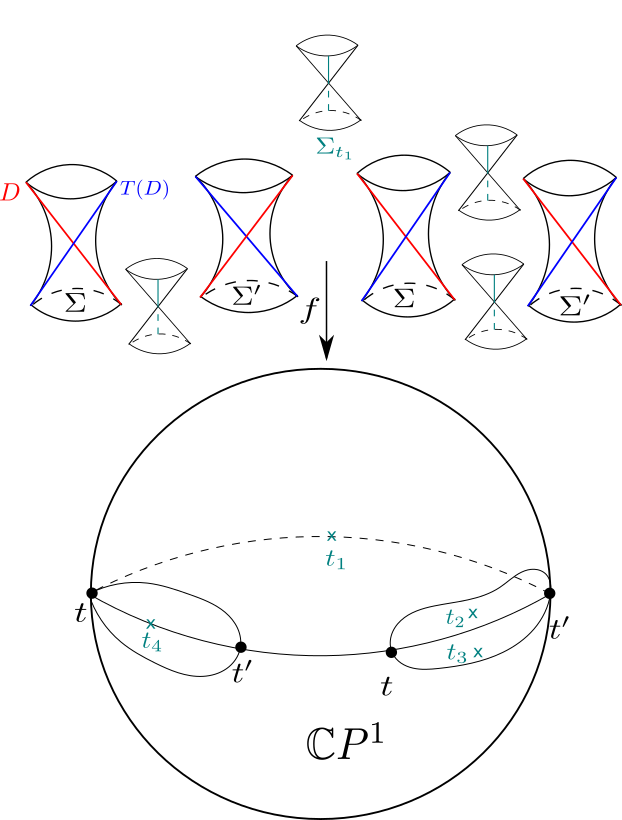
\includegraphics[scale=0.4]{figures/pencilquadric-article.png}
\caption{Example of a monodromy
transformation where the general fibers $\Sigma$ are quadric surfaces and the singular ones are quadric cones in $\cpp$.}
\label{fig-monodromy}
\end{figure}
   Let $(L_1,L_2)=([\C P^1\times\{\pt\}],[\{\pt\}\times \C P^1])$ be a basis of $H_2(\pp;\Z)$. The vanishing cycle is $S=L_1-L_2\in H_2(\pp;\Z)$.  It is straightforward to verify that, for any $(a, b) \in \mathbb{Z}^2$, the homology classes $aL_1+bL_2$ and $bL_1+aL_2$ are related by the monodromy transformation, that is, $bL_1+aL_2=T(aL_1+bL_2)$.
Thus, the monodromy interchanges the coefficients of $L_1$ and $L_2$. In other words, two classes $aL_1 + bL_2$ and $bL_1 + aL_2$ are equivalent under the equivalence relation induced by monodromy.    Therefore, for any non-singular fiber $\Sigma$ in this fibration, the quotient $H_2(\Sigma;\Z)/_{\sim}$ can be identified  with $H_2(\pp;\Z)\, /\, \langle L_1 - L_2 \rangle$. 
\end{example}

 
     From here on, we will use interchangeably the notation for homology classes in $H_2(\Sigma;\mathbb{Z})$ and  divisor classes in $\Pic(\Sigma)$, where $\Sigma$ is a del Pezzo surface. Given a divisor $D \in \Pic(\Sigma)$, we denote by $D|_{E,\Sigma} \in \Pic_{D.E}(E)$ its restriction to $E$. Here, $\Pic_{k}(E)$ denotes the group of divisor classes on $E$ of degree $k$ for any $k\in \mathbb{Z}$.  Since $K_\Sigma.S=0$, for $K_\Sigma$ the anti-canonical divisor of any non-singular surface $\Sigma$ in the pencil $\mathcal{Q}$ and $[E]=-K_\Sigma$, it follows that  the restriction of the vanishing cycle to $E$  lies in $\Pic_0(E)$.
    
 
\subsection{Enumeration on pencils of surfaces} \label{Sect-Pencils}
Recall that $E$ is the base locus of a pencil of surfaces in the linear system $|-\frac{1}{2}K_X|$ and $S$ is a generator of the kernel of the map $\psi$ as described after Lemma~\ref{Lemma-Vanishing.Cycle}.  Since $S.E=0$, for every divisor $D\in \Pic(\Sigma)$, the restrictions $D|_{E,\Sigma}$ and $T(D)|_{E,\Sigma}$ lie in $\Pic_{D.E}(E)$. Given any divisor $D$ on $\Sigma$ and its image under the monodromy transformation $T(D)$, we define the following holomorphic map:
\begin{align*}
    \phi\colon   \mathcal{Q}& \longrightarrow \Pic_{2D.E}(E)\\
    \Sigma_t &\longmapsto  (D+T(D))|_{E,\Sigma_t}, 
\end{align*}
where $D + T(D)$ is viewed as a divisor on $\Sigma_t$ and $|_{E, \Sigma_t}$ denotes its restriction to $E$.

\begin{lemma} \label{lem-constant.map}
The map $\phi$ is constant.
\end{lemma} 

\begin{proof}
  The pencil $\mathcal{Q}$ is parametrized by $\mathbb{C}P^1$, which is a compact Riemann surface of genus $0$, while $\Pic_{2D.E}(E)$ is an elliptic curve, that is, a compact Riemann surface of genus $1$. 
Any holomorphic map from a surface of lower genus to one of higher genus must be constant unless it is branched (which is not the case here). Therefore, the lemma follows. 
\end{proof}
  
We denote by $\overline{D}_{\phi}$ the divisor $(D+T(D))|_{E,\Sigma_t}$ or, equivalently, the divisor  $2D|_{E,\Sigma_t}+(D.S) S|_{E,\Sigma_t}$. The order~$2$ transformation $x \mapsto \overline{D}_{\phi} - x$ induces the following equivalence  relation on $\Pic_{D.E} (E)$:
$$x \sim y \quad \text{if and only if}\quad y=x \text{ or } y=\overline{D}_{\phi}-x.$$
We denote by $\overline{x}$ the equivalence class of $x$ under this relation.
Note that $\Pic_{D.E} (E)/_{x \sim \overline{D}_{\phi}-x}$ is the quotient of the elliptic curve $E$ by a fixed-point-free involution, and this quotient is holomorphically  
isomorphic to $\C {P}^1$.
We can define the following 
holomorphic map between Riemann spheres:
    \begin{align*}
    \phi_{\overline{D}}\colon  \mathcal{Q} &\longrightarrow \Pic_{D.E} (E)/_{x \sim \overline{D}_{\phi}-x}\\
    \Sigma_t &\longmapsto \overline{D|_{E,\Sigma_t}}, 
\end{align*}
where, for each $\Sigma_t \in \mathcal{Q}$, the class $\overline{D|_{E, \Sigma_t}}$ denotes the equivalence class of $D|_{E, \Sigma_t}$ in $\Pic_{D.E}(E)$ under the relation $x \sim \overline{D}_{\phi} - x$.

\begin{lemma} \label{lem-existence.of.L}
There exists a pair $\{L,T(L)\}\subset H_2(\Sigma;\Z)$ such that $(L.S)^2=1$. In particular, both classes $L$ and  $T(L)$ can be chosen to be effective. 
\end{lemma} 

\begin{proof}
According to \cite[Claim (6), p.~26]{demazure2006seminaire}, the vanishing cycle $S$ can always be expressed as the difference of two effective generators of $H_2(\Sigma; \mathbb{Z})$, and the monodromy transformation $T$ interchanges these two classes. Suppose that $S$ can be written as $L_1-L_2$, where $(L_1,L_2,L_3,\ldots, L_k)$ is a $k$-tuple of effective generators for $H_2(\Sigma;\Z)\cong \Z^k$. The intersection form on $H_2(\Sigma;\Z)$ implies that we can choose $L=L_2$ and $T(L)=L_1$, or \textit{vice versa}, so that $L.S = \pm 1$.  
\end{proof}

\begin{lemma}\label{lem-degree.phi(S)}
 One has $\deg (\phi_{\overline{S}})= 4$.
\end{lemma}

\begin{proof} 
  By Lemma~\ref{lem-existence.of.L}, for any pair of effective divisors $L$ and $T(L)$ on $\Sigma$ such that $L.S= \pm 1$, the pair $(L|_E, T(L)|_E)$  of their restrictions to the base locus $E$ determines a unique surface in the pencil $\mathcal{Q}$.  More precisely, if $L|_E \neq T(L)|_E$, this correspondence yields a non-singular surface in the pencil. Conversely, if $L|_E = T(L)|_E$, then $L$ and $T(L)$ restrict to the same divisor on $E$, which corresponds to a ramification point of the corresponding double covering of the parameter space. In this case, the corresponding surface in the pencil is singular, typically having an ordinary double point. Thus, the singular elements in the pencil are in bijection with the points where $L|_E = T(L)|_E$.  This relationship can be summarized by the following commutative diagram:
\begin{center}
 \begin{tikzcd}
\Pic_{L.E} (E) \arrow[r, "\hat{\pi}\colon x \mapsto \Sigma_x"] \arrow[d, "2:1"]
& \mathcal{Q} \arrow[dl, "\cong"] \\
\Pic_{L.E} (E)/_{x\sim \overline{L}_{\phi} -x}\rlap{\,,} & 
\end{tikzcd}
\end{center}
where $\hat{\pi}$ is a  ramified double covering map. Observe that $\hat{\pi}(\overline{L}_{\phi}-x)=\hat{\pi}(x)$, meaning that $\Sigma_{\overline{L}_{\phi}-x}=\Sigma_x$.
By analyzing the ramification points of $\hat{\pi}$, we obtain exactly four singular surfaces in the pencil $\mathcal{Q}$, which is consistent with Lemma~\ref{lem-4.singulars}. Furthermore, we have the following commutative diagram:
\begin{center}
 \begin{tikzcd}
&& \mathcal{Q} \arrow[d, "\phi_{\overline{S}}"] \arrow[dll] \\
\Pic_{L.E} (E)/_{x\sim \overline{L}_{\phi} -x}   \arrow[rr, "\overline{x}\mapsto \overline{\overline{L}_{\phi}-2 x}"]&&  \Pic_{0} (E)/_{y\sim -y}\rlap{\,.}
\end{tikzcd}
\end{center}

These diagrams together show that  each singular surface in the pencil $\mathcal{Q}$ corresponds to an element $x\in \Pic_{L.E}(E)$ such that $x=\overline{L}_{\phi}-x$, which is mapped to $\overline{0}\in \Pic_0(E)/_{y\sim -y}$. Consequently, the degree of the map $\phi_{\overline{S}}$  is exactly the number of singular surfaces in the pencil $\mathcal{Q}$, which is equal to $4$.
\end{proof}

\begin{corollary} \label{coro-isomorphism.pencil.picard}
Let $\{L,T(L)\}\subset H_2(\Sigma;\Z)$ be such that $(L.S)^2=1$. Then, the corresponding map $\phi_{\overline{L}}$ is an isomorphism. 
\end{corollary}

The following proposition is the main point for solving the \textit{$1$-dimensional problem} that we mentioned at the beginning of this section.


\begin{proposition} \label{Prop-degree.case.complex}
  Let $X$ be a $3$-dimensional del Pezzo variety such that
  $$\ker(\psi\colon  H_2(\Sigma;\mathbb{Z})\to H_2(X;\mathbb{Z}))\cong \Z,$$
  where $\Sigma\in \mathcal{Q}$ is a non-singular surface. Let $D\in \Pic(\Sigma)$ be a divisor. Let  $S\in \ker(\psi)$ be a generator.  Then, the map $\phi_{\overline{D}}$ has degree $(D.S)^2$.
\end{proposition} 


\begin{proof}
Consider the following commutative diagram of holomorphic maps between Riemann spheres:
\begin{equation}\tag{I}\label{I}
\centering
    \begin{tikzcd}
\mathcal{Q} \arrow[r, "\phi_{\overline{D}}"] \arrow[d, "\phi_{\overline{S}}"]
& \Pic_{D.E} (E)/_{x\sim \overline{D}_{\phi}-x} \arrow[d, "\theta_1"] \\
\Pic_{0} (E)/_{y\sim -y} \arrow[r, "\theta_2"]
& \Pic_{0} (E)/_{y\sim -y}\rlap{\,,}
\end{tikzcd}
\end{equation}
where
$$\theta_1(\overline{x})=\overline{\overline{D}_{\phi}-2x}\quad \text{and}\quad \theta_2(\overline{y})=(D.S)\overline{y}.$$
As a result, the following equality holds:
$$\deg\left(\phi_{\overline{D}}\right)\times \deg(\theta_1)=\deg\left(\phi_{\overline{S}}\right)\times \deg(\theta_2).$$
By Lemma~\ref{lem-degree.phi(S)}, we have $\deg (\phi_{\overline{S}})= 4$. In order to compute $\deg(\phi_{\overline{D}})$, we proceed to compute $\deg(\theta_1)$ and $\deg (\theta_2)$ as follows.

We first show that $\deg (\theta_2)= (D.S)^2$. Let $\overline{y_1} \in \Pic_{0} (E)/_{y\sim -y}$ (the quotient that is in the lower right corner of Diagram \eqref{I}). The degree of $\theta_2$ can be expressed as
$$\deg(\theta_2)=\left|\left\{\overline{y}\in \Pic_{0} (E)/_{y\sim -y} \; : \; (D.S)\overline{y}=\overline{ y_1}\right\}\right|.$$
The commutative diagram
\begin{center}
    \begin{tikzcd}
\Pic_{0} (E) \arrow[r, "y\mapsto (D.S)y"] \arrow[d, "2:1"]
& \Pic_{0} (E) \arrow[d, "2:1"] \\
\Pic_{0} (E)/_{y\sim -y} \arrow[r, "\theta_2"]
& \Pic_{0} (E)/_{y\sim -y}
\end{tikzcd}
\end{center}
 implies that $\deg(\theta_2)$ is exactly the number of solutions $y\in \Pic_0(E)$ to the equation $(D.S)y=y_1$ in $\Pic_0(E)$, in  which the divisor $y_1$ is given. Moreover, any two solutions $y$ to this equation differ by a torsion point of order $D.S$. This equation then has exactly $(D.S)^2$ solutions $y$. Hence, $\deg(\theta_2)=(D.S)^2$, as required.

We now show that  $\deg (\theta_1)= 4$ in a similar way. Let $\overline{y_1} \in \Pic_{0} (E)/_{y\sim -y}$ (the quotient that is in the lower right corner of Diagram \eqref{I}. The degree of $\theta_1$ can be expressed as
$$\deg(\theta_1)=\left|\left\{\overline{x}\in \Pic_{D.E} (E)/_{x\sim \overline{D}_{\phi} -x} \; : \; \overline{ \overline{D}_{\phi}-2x}=\overline{ y_1}\right\}\right|.$$
The commutative diagram
\begin{center}
    \begin{tikzcd}
\Pic_{D.E} (E) \arrow[r, "x\mapsto \overline{D}_{\phi}-2x"] \arrow[d, "2:1"]
& \Pic_{0} (E) \arrow[d, "2:1"] \\
\Pic_{D.E} (E)/_{x\sim \overline{D}_{\phi} -x} \arrow[r, "\theta_1"]
& \Pic_{0} (E)/_{y\sim -y}
\end{tikzcd}
\end{center}
implies that $\deg(\theta_1)$ is exactly the number of solutions $x\in \Pic_{D.E}(E)$ to the equation $\overline{D}_{\phi}-2x=y_1$ in $\Pic_0(E)$, where the two divisors $y_1$ and $\overline{D}_{\phi}$ are given. Moreover, any two solutions $x$ to this equation differ by a torsion point of order $2$. This equation then has exactly $2^2$ solutions $x$.  Hence, $\deg(\theta_1)=4$, as required.
This completes the proof of the proposition.
\end{proof}

\subsection{Real pencils of real del Pezzo surfaces}
Throughout this subsection,  we restrict our attention to a real $3$-dimensional del Pezzo variety $(X,\tau)$  such that $\ker(\psi) \cong \Z$, where $\Sigma \in |-\frac{1}{2}K_X|$ is a non-singular surface, and the surjection $\psi\colon  H_2(\Sigma;\mathbb{Z})	\twoheadrightarrow H_2(X;\mathbb{Z})$ is induced by the inclusion $\Sigma\hookrightarrow X$. Henceforth, the notions of vanishing cycle and generator of $\ker (\psi)$ may be used interchangeably (see Lemma~\ref{Lemma-Vanishing.Cycle}). Let $\mathcal{Q}$ denote a pencil of surfaces in the linear system $|-\frac{1}{2}K_X|$. Let the elliptic curve $E$ be its base locus. Recall that $E$ realizes the homology class $\frac{1}{4}K_X^2$ (see Proposition~\ref{Prop-E.is.elliptic}). Now suppose  that both the curve $E$ and the pencil $\mathcal{Q}$ are real with non-empty real parts. We first examine certain properties of the real pencil $\mathcal{Q}$ that distinguish them from the complex case.

\subsubsection{Properties of real pencils of real surfaces}

 
\begin{lemma} \label{lem-surfaces.in.real.pencil}
The surfaces in the real pencil $\mathcal{Q}$ containing a real rational curve in $(X,\tau)$ are in the real part $\R \mathcal{Q}$ of this pencil.
\end{lemma}

\begin{proof}
  Let $C$ be a real rational curve in $(X,\tau)$. Suppose that the surface $\Sigma\in \mathcal{Q}$ contains $C$. Since $\mathcal{Q}$ is a real pencil, we have $\tau(\Sigma)\in \mathcal{Q}$. Since $C$ is real, we have $\tau(C)=C$.  If $\Sigma\notin \R \mathcal{Q}$, \textit{i.e.}, $\tau(\Sigma)\neq \Sigma$, then $C\subset (\Sigma\cap \tau(\Sigma))=E$, which is not possible since $C$ is a rational curve. Thus, by contradiction  $\tau(\Sigma)=\Sigma$. In other words, $\Sigma$ is in the real part of the pencil $\mathcal{Q}$.
\end{proof}

Note that if $(\Sigma_1,\tau|_{\Sigma_1})$ and $(\Sigma_2,\tau|_{\Sigma_2})$ are two real non-singular surfaces in $\R \mathcal{Q}$ such that $\Sigma_2$ is a surgery of $\Sigma_1$ along the vanishing cycle (as formalized in \cite{brugalle2018surgery}), then the Euler characteristics of the real parts of these two surfaces differ by~$2$. Suppose that $\chi(\R \Sigma_2)=\chi(\R \Sigma_1)+ 2$. Also note  from \cite{brugalle2018surgery} that the vanishing cycle class $S$ in $H_2(\Sigma_1;\Z)$ is $\tau|_{\Sigma_1}$-anti-invariant if and only if it is $\tau|_{\Sigma_2}$-invariant.  Let $\alpha \in \{D,T(D)\}$. We say that $\alpha$ is $\tau|_{\Sigma_t}$-anti-invariant if we have both
$\tau|_{\Sigma_t*}(D)=-D$ and
$\tau|_{\Sigma_t*}(T(D))=-T(D)$.

\begin{proposition} \label{prop-tau.vs.mu}
Let $d\in H^{-\tau}(X;\Z)$. Let $(\Sigma_t,\tau|_{\Sigma_t}) \in \R \mathcal{Q}$ be a real del Pezzo surface containing a real rational curve in $X$ $(t\in {\R})$, and let $\psi_t\colon  H_2(\Sigma_t;\mathbb{Z})\rightarrow H_2(X;\mathbb{Z})$ be the surjective map  induced from the inclusion $\Sigma_t\hookrightarrow X$. Let $\alpha \in \{D,T(D)\}\subset \psi_t^{-1}(d)$ be such that $D.S\neq 0$. In the real surface $(\Sigma_t,\tau|_{\Sigma_t})$, the vanishing cycle is $\tau|_{\Sigma_t}$-anti-invariant if and only if $\alpha$ is $\tau|_{\Sigma_t}$-anti-invariant.
\end{proposition}  

\begin{proof}
The sufficient condition follows directly. Indeed, suppose that
$$\begin{cases}
\tau|_{\Sigma_t*}(D)=-D,\\
\tau|_{\Sigma_t*}(T(D))=-(D+(D.S)S)
\end{cases}$$
hold. Then, $$(D.S)\tau|_{\Sigma_t*}(S)=\tau|_{\Sigma_t*}(T(D)-D)=-(D.S)S.$$
If $D \cdot S \neq 0$, we conclude that $\tau|_{\Sigma_t*}(S) = -S$; that is, $S$ is $\tau|_{\Sigma_t}$-anti-invariant. This completes the proof of the sufficiency.

The necessary condition is established in the following two steps.

\textit{Step 1. We show that $\tau|_{\Sigma_t*}(\{D,T(D)\})=\{-D,-T(D)\}$.}
Suppose that $\alpha=D$. It suffices to prove that if $D$ satisfies $\psi_t(D)=d\in H^{-\tau}(X;\Z)$, then one of the following holds:
\begin{enumerate}
    \item $\tau|_{\Sigma_t*}(D)=-D$; \textit{i.e.}, $D$ is $\tau|_{\Sigma_t}$-anti-invariant.
    \item $\tau|_{\Sigma_t*}(D)=-(D+(D.S)S)$, where $S$ is a generator of $\ker(\psi_t)$.
\end{enumerate}
Indeed, since $\tau_* (d)=-d$, we have $\tau_*(\psi_t(D))=-\psi_t (D)$. Because $\psi_t\circ\tau|_{\Sigma_t*}=\tau_*\circ \psi_t$, it follows that $\psi_t (\tau|_{\Sigma_t*}(D)+D)=0$. Moreover, since $\ker (\psi_t) =\Z S$, there exists an integer $k\in \Z$ such that $\tau|_{\Sigma_t*}(D)+D=kS$. The intersection form is preserved under $\tau|_{\Sigma_t*}$; that is, $(\tau|_{\Sigma_t*}(D))^2=D^2$. Thus, $k$ must be either $0$ or $-D.S$. This completes the first step.


\textit{Step 2. We show that if $(\Sigma_t,\tau|_{\Sigma_t})$ is  such that the vanishing cycle $S$ is $\tau|_{\Sigma_t}$-anti-invariant in $H_2(\Sigma_t; \Z)$, then both $D$ and $T(D)$ must be $\tau|_{\Sigma_t}$-anti-invariant. } Suppose, toward a contradiction, that $\tau|_{\Sigma_t*}(D)=-T(D)$. One has $\tau|_{\Sigma_t*}(D)=-D-(D.S)S=\tau|_{\Sigma_t*}(T(D))-(D.S)S$. This implies that 

$$\tau|_{\Sigma_t*}(T(D))-\tau|_{\Sigma_t*}(D)=(D.S)S.$$
Moreover, $$\tau|_{\Sigma_t*}(T(D))=\tau|_{\Sigma_t*}(D+(D.S)S)=\tau|_{\Sigma_t*}(D)+(D.S) \tau|_{\Sigma_t*}(S).$$
Comparing the two expressions, we obtain $S=\tau|_{\Sigma_t*}(S)$. This means that $S$ is not $\tau|_{\Sigma_t}$-anti-invariant, which contradicts our assumption. Thus, the second step is complete, and the proposition follows.
\end{proof}

As a consequence, the enumerative problem of counting real curves representing $\tau$-anti-invariant classes in $X$ can be reduced to the enumerative problem of counting real curves representing $\tau|_{\Sigma_t}$-anti-invariant  classes in some surface $\Sigma_t$. The latter problem is, in general, simpler and has been extensively studied in the literature on real enumerative geometry.

To make a meaningful comparison between these two real enumerative problems, we analyze the real base locus $E$ as in the complex case. It is well known that the choice of a point $x_0\in E$ induces an isomorphism $E\cong \Pic_k(E)$  for any $k\in \mathbb{Z}$. Since $E$ is a real elliptic curve and $\R E\neq \emptyset$, the real parts  $\R E$ and $\R \Pic (E)$ have the same topological type. Consequently, there exists a homeomorphism $\R E \simeq \R \Pic_k(E)$ for any $k\in \mathbb{Z}$. Assume that $x_0\in \R E$. The real part $\R E$ is either connected or disconnected with two connected components. In the former case, we write $\mathbb{R} E =\mathbb{S}^1$. In the latter case, we write $\mathbb{R} E =\mathbb{S}^1_0\sqcup \mathbb{S}^1_1$ and assume that $x_0\in\mathbb{S}^1_0$. We refer to $\mathbb{S}^1_0$ as the \textit{pointed component} and $\mathbb{S}^1_1$ as the \textit{non-pointed component} of $\R E$.

 
 

Let $\underline{x}_{d}$ be a real configuration of $|D.E|$ points on $E$. Suppose that $\alpha|_{E,\Sigma_t}=[\underline{x}_{d}]$ in $\Pic_{D.E}(E)$, where $\alpha$ is as in Proposition~\ref{prop-tau.vs.mu}. 
We consider the  maps
    \begin{align*}
    \mu_t\colon \Pic(\Sigma_t)&\lra \Pic(\Sigma_t)\\
    \sum_i n_i [C_i]&\longmapsto \sum_i n_i \left[\tau|_{\Sigma_t}(C_i)\right]
\end{align*}
and
\begin{align*}
    \mu_E\colon \Pic(E)&\lra \Pic(E)\\
    \sum_i n_i [P_i]&\longmapsto \sum_i n_i \left[\tau|_{E}(P_i)\right].
\end{align*}
The restriction of a divisor $D=\sum_i n_i [C_i]\in \Pic(\Sigma_t)$ to $\Pic(E)$ is given by $$D|_{E,\Sigma_t}=\sum_i n_i [C_i\cap E].$$ 
The restriction of $\Pic(\Sigma_t)$ to $\Pic(E)$ induces the following commutative diagram:
 \begin{center}
    \begin{tikzcd}
\Pic(\Sigma_t) \; \; \;  \arrow[rr, "\mu_t"] \arrow[d]
&& \; \; \;  \Pic(\Sigma_t)\arrow[d] \\
\Pic(E)  \; \; \;  \arrow[rr, "\mu_E"]
&& \; \; \;  \Pic(E)\rlap{.}
    \end{tikzcd}
        \end{center}
 
     \begin{lemma} \label{lem-anti-invariant.and.real.divisors}
         If the class $D$ is $\tau|_{\Sigma_t}$-anti-invariant, then its restriction $D|_{E,\Sigma_t}$ lies in $\R \Pic(E)$.
     \end{lemma}

     \begin{proof}
   We show that if $D$ is 
$\tau|_{\Sigma_t}$-anti-invariant, then  $\mu_E(D|_{E,\Sigma_t})=D|_{E,\Sigma_t}$.  Indeed, since the involution $\tau$ reverses the orientation, meaning that $\mu_t=-\tau|_{\Sigma_t*}$, one has $D|_{E,\Sigma_t}=\mu_t(D)|_{E,\Sigma_t}$. The above commutative diagram implies that $\mu_E(D|_{E,\Sigma_t})=\mu_t(D)|_{E,\Sigma_t}$. Hence, the lemma follows.
\end{proof}

 
Given $D \in \Pic(\Sigma_t)$, we consider the following ramified double covering:
\[
\pi\colon  \Pic(E) \longrightarrow \Pic(E) \big/ \sim, \quad x \longmapsto \overline{x},
\]
where the equivalence relation is defined by $x \sim \overline{D}_{\phi} - x$. The critical points of the map $\pi$ are precisely the solutions to the equation $2x = \overline{D}_{\phi}$ in $\Pic(E)$. There exists a homeomorphism
\[
\mathbb{R} \left( \Pic(E) \big/ \sim \right) \simeq \mathbb{S}^1.
\]
Moreover, the preimage of the real locus under $\pi$ is given by
\[
\pi^{-1} \left( \mathbb{R} \left( \Pic(E) \big/ \sim \right) \right )
= \left\{\, (x,\, \overline{D}_{\phi} - x) \; : \; x \in \mathbb{R}\Pic(E) \, \right\}
\cup \left\{\, (y,\, \tau|_E(y)) \; : \; y \in \Pic(E) \setminus \mathbb{R}\Pic(E),\; y + \tau|_E(y) = \overline{D}_{\phi} \, \right\},
\]
where $\tau|_E$ denotes the real structure on $E$. The two types of real divisors on  $\mathbb{R}(\Pic(E)/_{x \sim \overline{D}_{\phi}-x})$ are as illustrated in  Figure~\ref{fig-RealElliptic}. 

\begin{figure}[ht!]
\centering
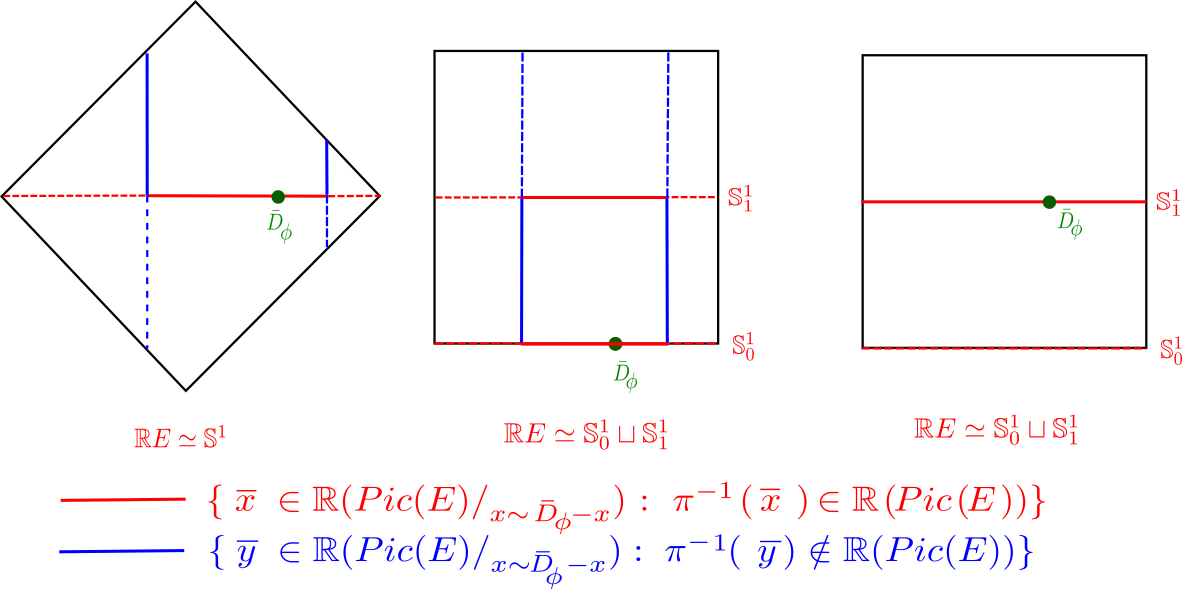
\includegraphics[scale=0.4]{figures/RealElliptic.png}
\caption{Real divisors in the Picard group $\mathbb{R}(\Pic(E)/_{x \sim \overline{D}_{\phi}-x})$ of a real elliptic curve with non-empty real part.}
\label{fig-RealElliptic}
\end{figure}


 
\subsubsection{Enumerations on real pencils of real del Pezzo surfaces}
We keep the same notation as in  Section~\ref{Sect-Pencils}: the vanishing cycle  $S$ of the Lefschetz fibration induced from the pencil $\mathcal{Q}$, the constant map $\phi$ whose image is the divisor  $\overline{D}_{\phi}=(2D+(D.S)S)|_{E,\Sigma_t}$ in  $\Pic_{2D.E} (E)$, which is independent of $\Sigma_t \in \mathcal{Q}$, and the degree $(D.S)^2$ map $\phi_{\overline{D}}$ (see Proposition~\ref{Prop-degree.case.complex}). 

Assume that $\{L,T(L)\}\subset H_2(\Sigma_t;\Z)$ is as in  Lemma~\ref{lem-existence.of.L}. Recall, in particular, that $\overline{L}_{\phi}$ is  in $\Pic_{2L.E}(E)$ and $\phi_{\overline{L}}$ is an isomorphism (Corollary~\ref{coro-isomorphism.pencil.picard}). As previously shown, the divisor $\overline{D}_{\phi}$ is real, for every class $D \in H^{-\tau}(\Sigma_t;\Z)$ (see Lemma~\ref{lem-anti-invariant.and.real.divisors}). In particular, the divisor $\overline{L}_{\phi}$ is real, and both $\phi_{\overline{D}}$ and $\phi_{\overline{L}}$ are real maps.
Let $\mathcal{R}(\underline{x}_d)$ be a set of real irreducible rational curves in $X$ representing a given homology class $d\in H^{-\tau}(X;\Z)$ and passing through a real configuration $\underline{x}_d$ of $k_d=\frac{1}{2}c_1(X)\cdot d$ points on $E$.


\begin{lemma} \label{lem-constant.divisor.L.D}
The divisor $(D-|D.S|L)|_{E,\Sigma_t}$, which has degree $(D.E)-|D.S|(L.E)$ in $\Pic(E)$, is denoted by $\phi(\overline{L},\overline{D})$ and does not depend on the choice of the surface $\Sigma_t$ in the pencil $\mathcal{Q}$.
\end{lemma}


\begin{proof}
Clearly, the divisor  $(D-|D.S|L)|_{E,\Sigma_t}$ has degree $(D.E)-|D.S|(L.E)$ in $\Pic(E)$. Without loss of generality, suppose that $D.S> 0$. We have
  \begin{align*}
      2\left(D-(D.S)L\right)|_{E,\Sigma_t} &= \left(2D-2(D.S)L\right)|_{E,\Sigma_t}\\
      &= \left((2D+(D.S)S)-(D.S) (2L+S)\right) |_{E,\Sigma_t}.
  \end{align*}
   
As previously shown, both $(2L+S)|_{E,\Sigma_t}=\overline{L}_{\phi}$ and $(2D+(D.S)S)|_{E,\Sigma_t}=\overline{D}_{\phi}$ are constant with respect to $\Sigma_t$. Consequently, the divisor $ 2\left(D-(D.S)L\right)|_{E,\Sigma_t}$ does not depend on the choice of $\Sigma_t$. Therefore, by continuity, the divisor $ \left(D-(D.S)L\right)|_{E,\Sigma_t}$  is also independent of $\Sigma_t$. 
\end{proof}

The next proposition is the main ingredient to solving the \textit{$1$-dimensional real problem} of Theorem~\ref{Theorem2-W}.

\begin{proposition} \label{prop-corresponding.surface.picE}
Let $\Sigma \in \mathcal{Q}$ be a fixed real non-singular surface.
Let $d\in H^{-\tau}(X;\Z)$, and let $\alpha$ be an element of 
$\{D,T (D)\}\subset \psi^{-1}(d)$. Then, for any real surface $(\Sigma_t, \tau|_{\Sigma_t}) \in \mathbb{R} \mathcal{Q}$ containing a curve in the set $\mathcal{R}(\underline{x}_d)$, the corresponding vanishing cycle is $\tau|_{\Sigma_t}$-anti-invariant.

Furthermore, such real surfaces correspond to the real solutions $l\in \R \Pic(E)$ of the equation
\begin{equation}\label{eq-solutions.in.PicE}
    |D.S|l=[\underline{x}_d]-\phi\left(\overline{L},\overline{D}\right),
\end{equation}
where $[\underline{x}_d]$ and $\phi(\overline{L}, \overline{D})$  are as previously defined.
\end{proposition}

\begin{proof}
  The first assertion follows directly from the fact that if the vanishing cycle is not $\tau|_{\Sigma_t}$-anti-invariant, then $D\notin  H_2^{-\tau}(\Sigma_t;\Z)$ for any $D\in H_2(\Sigma_t;\Z)$.
  
  We now address the second assertion. Since the equality $D.S=-T(D).S$ holds, we may assume without loss of generality that $D.S> 0$.
   Then, one has
  $$\phi\left(\overline{L},\overline{D}\right)=\left(D-(D.S)L\right)|_{E,\Sigma_t}=\left(D+(T(D).S)L\right)|_{E,\Sigma_t}.$$ 
 
  Let $\Sigma_t \in \mathcal{Q}$  be a surface containing a curve in  $\mathcal{R}(\underline{x}_d)$, and suppose that this curve represents the homology class $D\in H_2^{-\tau}(\Sigma_t;\Z)$. Then, $[\underline{x}_d]=D|_{E,\Sigma_t}$ is a real divisor in $\Pic_{D.E}(E)$.
    

We can write  $D=(D.S)L+D-(D.S)L$. Restricting to $E$, and noting that $L$ is also $\tau|_{\Sigma_t}$-anti-invariant, we obtain the following equation in $\Pic(E)$:
  $$\left[\underline{x}_d\right]=(D.S)L|_{E,\Sigma_t}+\left(D-(D.S)L\right)|_{E,\Sigma_t}.$$
 By Lemma~\ref{lem-constant.divisor.L.D}, the divisor $\left(D-(D.S)L\right)|_{E,\Sigma_t}=\phi(\overline{L},\overline{D})$ does not depend on the choice of the surface $\Sigma_t$ in the pencil. 
 Therefore, for every surface $\Sigma_t \in \mathcal{Q}$ containing a curve in $\mathcal{R}(\underline{x}_d)$ of homology class $D\in H_2^{-\tau}(\Sigma_t;\Z)$ where $D.S> 0$, the following equation holds in $\Pic(E)$:
 $$(D.S)L|_{E,\Sigma_t}=[\underline{x}_d]-\phi\left(\overline{L},\overline{D}\right).$$
 Consequently, for every real surface $\Sigma_t \in  \R \mathcal{Q}$, on which a curve in $\mathcal{R}(\underline{x}_d)$ represents a $\tau|_{\Sigma_t}$-anti-invariant class $\alpha\in \{D,T (D)\}$, we have
 \begin{equation} \label{eq-proof-eq-solutions.in.PicE}
     (|D.S|L)|_{E,\Sigma_t}=[\underline{x}_d]-\phi(\overline{L},\overline{D})
 \end{equation}
  in $ \Pic(E)$. Moreover, the map
  $$   \phi_{\overline{L}}\colon  \mathcal{Q} \overset{\lowcong}\lra \Pic_{L.E} (E)/_{x\sim \overline{L}_{\phi}-x}, \quad    \Sigma_t \longmapsto \overline{L|_{E,\Sigma_t}}$$
   is a real isomorphism. Together with the remarks on real structures on the pencil $\mathcal{Q}$ and on the quotient of the Picard group of its base locus, this implies that such real surfaces $\Sigma_t \in  \R \mathcal{Q}$ are precisely the real solutions in  $\R \Pic(E)$ to Equation (\ref{eq-proof-eq-solutions.in.PicE}). The proposition is thus established.
  \end{proof}

\section{Rational curves on del Pezzo varieties of dimension 3 and 2: Relationship } \label{Section-ratcurve}
Recall from the last section that a non-singular element $\Sigma\in |-\frac{1}{2}K_X|$ is a non-singular del Pezzo surface, where $X$ is a del Pezzo variety of dimension~$3$. Also recall  that $\psi\colon  H_2(\Sigma;\mathbb{Z})\to H_2(X;\mathbb{Z})$ is the surjective map induced by the inclusion $\Sigma\hookrightarrow X$.

 
 
 In this section, we continue to use the notation $\mathcal{Q}$ to denote a pencil of surfaces in the linear system $|-\frac{1}{2}K_X|$, whose base locus is the elliptic curve $E$ representing the class $\frac{1}{4}K_X^2$.  Let $d\in H_2(X;\mathbb{Z})$ and $k_d=\frac{1}{2}c_1(X)\cdot d$. Let $D\in H_2(\Sigma;\mathbb{Z})$ and $k_D=c_1(\Sigma)\cdot D-1$. We proceed to analyze the case where the configuration points are constrained to lie on the elliptic curve $E$. As a first step, we  establish a generalization of a result due to J.~Koll\'ar (Proposition~\ref{Prop-Kollar}). Subsequently, we demonstrate that the selected specialized configuration gives us the genus $0$ Gromov--Witten invariants of the surface $\Sigma$ (see Proposition~\ref{Prop.Modulispace1}, Corollary~\ref{Corollary.Modulispace1}) and of the variety~$X$ (see Proposition~\ref{Prop.Modulispace2}). As a result, this allows us to relate $\GW_X(d)$ to $\GW_\Sigma(D)$.

\subsection{Specifications of configuration of points} \label{SectionSpecificationConfiguration}
 \begin{lemma} \label{lemkDandkd}
Given a $3$-dimensional del Pezzo variety $X$, if\,  $\Sigma\in |-\frac{1}{2}K_X|$ is a non-singular surface and $D\in \psi^{-1}(d)$, then one has $k_D=k_d-1$. 
\end{lemma}

 \begin{proof}
   By the Poincar\'e duality $\tfrac{1}{2}c_1(X)=\PD(-\tfrac{1}{2}K_X)$ and by the hypothesis that $\Sigma\in |-\tfrac{1}{2}K_X|$ is non-singular, we have
   $$k_d=\tfrac{1}{2}c_1(X)\cdot d=[\Sigma]. d .$$
By the adjunction formula, by the hypothesis $D\in \psi^{-1}(d)$ 
and by the Poincar\'e duality $c_1(\Sigma) =\PD(-K_\Sigma)$, we obtain
\begin{equation*}
[\Sigma].d=-K_\Sigma.D=k_D+1.
\end{equation*}
Hence, the lemma follows. 
\end{proof}

  The following proposition generalizes \cite[Proposition 3]{kollar2015examples} by J.~Koll\'ar for the case $\cpp$.

\begin{proposition} \label{Prop-Kollar}
Let $d\in H_2(X;\Z)$, and let  $\underline{x}_d$ be a configuration of\, $k_d=\tfrac{1}{2}c_1(X)\cdot d$ points in general position in the base locus $E$ of pencil $\mathcal{Q}$ of surfaces in the linear system $|-\frac{1}{2}K_X|$. Let $\mathcal{C}(\underline{x}_d)$ be the set of \textit{connected algebraic curves of arithmetic genus $0$ representing the homology class $d$ and passing through $\underline{x}_d$}. Then every curve in $\mathcal{C}(\underline{x}_d)$ is irreducible and is contained in some non-singular surface of\,  $\mathcal{Q}$.
 \end{proposition}
 
 \begin{remark}
     Such non-singular surfaces correspond to solutions $l\in \Pic(E)$ of Equation (\ref{eq-solutions.in.PicE}).
 \end{remark}

 \begin{proof}
Let $C_d$ be a curve in the set $\mathcal{C}(\underline{x}_d)$. We prove the following claims.

\begin{claim}{1}\label{claim3.2-1}
Suppose that $C_d$ is irreducible. Then,  the whole curve $C_d$ has to be contained in some non-singular surface of the pencil $\mathcal{Q}$.
\end{claim}

The first observation is that any point of $C_d\setminus\underline{x}_d$ is contained in some  surface, which is denoted by $\Sigma_t$, of the pencil $\mathcal{Q}$. Then, the number of intersection points between $C_d$ and  $\Sigma_t$ is at least $\frac{1}{2}c_1(X)\cdot d$. By B\'ezout's theorem, the whole curve $C_d$ has to be contained in this surface. We subsequently show that such a surface $\Sigma_t$ is non-singular provided that the chosen points of $\underline{x}_d$ are sufficiently generic. Indeed, suppose, toward a contradiction, that the curve $C_d$ (passing through the configuration $\underline{x}_d$ on $E$) is contained in a singular surface $\Sigma_{\sing}$ of the pencil $\mathcal{Q}$. Let $\rank(\Pic(\Sigma_{\sing}))=k-1$, where  $k\geq 2$. Note that  $\rank(\Pic(\Sigma_{\sing}))=\rank(\Pic(\Sigma))-1$, where $\Sigma$ is a non-singular surface in $\mathcal{Q}$. Let $(L_1,L_2\ldots,L_k)$ be a basis of $ H_2(\Sigma;\Z)$, such that the vanishing cycle $S$ satisfies $S=L_1-L_2\in H_2(\Sigma;\Z)$. Let $(\tilde{L}_{12},\tilde{L}_3\ldots,\tilde{L}_k)$ be a basis of $ H_2(\Sigma_{\sing};\Z)$. Consider the  homomorphism given by
\begin{align*}
    \gamma\colon H_2(\Sigma;\Z_2)&\lra H_2(\Sigma_{\sing};\Z)\\
    L_1-L_2& \longmapsto 0 \\
    L_1+L_2& \longmapsto \tilde{L}_{12}\\
    L_i & \longmapsto \tilde{L}_i,\quad \forall i \in \{3,\ldots,k\}.
\end{align*}

Suppose that the curve $C_d$ represents the homology class $[C_d]=\alpha_{1}\tilde{L}_{12}+\alpha_3 \tilde{L}_3+\cdots + \alpha_k \tilde{L}_k$ in $H_2(\Sigma_{\sing};\Z)$. By this morphism, such a curve realizes the homology class $D=\alpha_{1}L_{1}+\alpha_1 L_2+\alpha_3 L_3+\cdots + \alpha_k L_k$ in $H_2(\Sigma;\Z)$. By Equation (\ref{eq-solutions.in.PicE}) in Proposition~\ref{prop-corresponding.surface.picE}, and by the remark that $D.S=0$, we have
$[\underline{x}_d]=-\phi (\overline{L},\overline{D})$ in $\Pic_{k_d}(E)$. This contradicts the genericity of the configuration $\underline{x}_d$. 

To prove that $C_d$ is irreducible, we argue by contradiction, making use of the following three claims. Suppose that $C_d$ can be decomposed into $n$ ($n\geq 0$) irreducible rational curves $C_{d_i}$, that is, $C_d=\bigcup_{i=1}^{n} C_{d_i}$, where $C_{d_i}$ realizes a homology class $d_i\in H_2(X;\mathbb{Z})$ provided that $\sum_{i=1}^{n}d_i=d$, and  $C_d$  passes through $\underline{x}_{d_i}$ such that $\bigcup_{i=1}^{n}\underline{x}_{d_i}=\underline{x}_d$.


\begin{claim}{2A}\label{claim2}
  Each component curve $C_{d_i}$ passes though exactly $k_{d_i}=\frac{1}{2}c_1(X)\cdot d_i$ points of configuration $\underline{x}_d$.
  \end{claim} 
Indeed, suppose that there exists a component of $C_d$, denoted by $C_{d_1}$, passing through more than $\frac{1}{2}c_1(X)\cdot d_1$ points of $\underline{x}_d$. Then the curve $C_{d_1}$ intersects with every surface of the pencil $\mathcal{Q}$ at more than $\frac{1}{2}c_1(X)\cdot d_1$ points. By B\'ezout's theorem, this implies that $C_{d_1}$ must be contained in every surface of the pencil $\mathcal{Q}$, and hence $C_{d_1} = E$. This is impossible since $C_{d_1}$ is a genus $0$ curve. Hence, every component curve $C_{d_i}$ passes through a configuration $\underline{x}_{d_i}$ of exactly $k_{d_i}$
points of $\underline{x}_d$. As a consequence, the different $C_{d_i}$ passes though different points of $\underline{x}_d$ for all $i$; \textit{i.e.}, $\bigsqcup_{i=1}^{n}\underline{x}_{d_i}=\underline{x}_d$ and $\sum_{i=1}^{n}k_{d_i}=k_d$, where $k_d$ and $k_{d_i}$ are the corresponding integers of the classes $d$ and $d_i$, respectively.

\begin{claim}{2B}\label{claim2B}
  The reducible curve $C_d=\bigcup_{i=1}^{n} C_{d_i}$ is contained in one non-singular surface of the pencil $\mathcal{Q}$.
\end{claim}
Note that the curve $C_d$ is connected. Suppose, toward a contradiction, that two component curves $C_{d_i}$ and $C_{d_j}$, whose intersection is not empty, are contained in two different surfaces $\Sigma_i\neq \Sigma_j$ of the pencil $\mathcal{Q}$. It follows that $\emptyset \neq C_{d_i}\cap C_{d_j}\subset \Sigma_i\cap\Sigma_j=E$. This is in contradiction with Claim~\ref{claim2}. 
Hence the reducible curve $C_d$ is contained in only one  surface of the pencil $\mathcal{Q}$. Moreover, such a surface is non-singular by the genericity of the chosen configuration. One can suppose that the curve $C_d$ is contained in $\Sigma_t\in \mathcal{Q}$ and  present its homology class as $[C_d]=\sum_{i=1}^{n} [C_{d_i}]\in H_2(\Sigma_t;\Z)$.


\begin{claim}{2C}\label{lem44}
  If the configuration $\underline{x}_d$ is generic, then the curve $C_d$ is irreducible.
\end{claim}

We prove this claim  by contradiction as well. 
Fix an integer $k_{d_1}$ such that $0<k_{d_1}<k_d$. Let $\underline{x}_{d_1}\subsetneq \underline{x}_d$ be a strict subconfiguration consisting of points on $E$ such that its cardinality is equal to $k_{d_1}$. Suppose that the curve $C_{d_1}$ realizes a homology class $D_{1}$ in $H_2(\Sigma;\Z)$. By the proof of Proposition~\ref{prop-corresponding.surface.picE}, we have
$$\left[\underline{x}_{d_1}\right]=|D_1\cdot S|l+\phi\left(\overline{L},\overline{D}_1\right).$$
Together with Equation (\ref{eq-solutions.in.PicE}) in Proposition~\ref{prop-corresponding.surface.picE}, we get the following equation in $\Pic(E)$: 
\begin{equation}\label{eq3.2}
    |D\cdot S|\left[\underline{x}_{d_1}\right]=|D_1\cdot S|\left[\underline{x}_d\right]-|D_1\cdot S|\phi \left(\overline{L},\overline{D}\right)+|D\cdot S|\phi\left(\overline{L},\overline{D}_1\right).
\end{equation}
By Lemma~\ref{lem-constant.divisor.L.D}, both $\phi (\overline{L},\overline{D})$ and $\phi(\overline{L},\overline{D}_1)$ are fixed divisors in $\Pic(E)$. Hence, Equation \eqref{eq3.2} is possible only when $\underline{x}_{d_1}=\underline{x}_{d}$. Therefore, there are no reducible curves $C_d$ for a general choice of the configuration $\underline{x}_{d}$.  
This last claim finishes our proof of Proposition~\ref{Prop-Kollar}.
    \end{proof}

\subsection{Moduli spaces and enumeration of balanced rational  curves}
In this technical part, we show, by specializing our configuration of points, that we can recover the genus~$0$ Gromov--Witten invariants of the $3$-dimensional del Pezzo variety $X$ and of a non-singular del Pezzo surface in $|-\frac{1}{2}K_X|$; see \cite[Section 5]{brugalle2016pencils}. 

\subsubsection{Moduli spaces of stable maps and balanced rational curves} 

Consider the moduli space $\mathcal{M}_{0,k_d}(X,d)$  of irreducible genus $0$ $k_d$-pointed stable maps
$$f\colon \left(\mathbb{C}P^1;p_1,\ldots,p_{k_d}\right)\lra X$$
of homology class $d\in H_2(X;\Z)$. Let $\mathcal{M}^*_{0,k_d}(X,d)$ denote the subspace of $\mathcal{M}_{0,k_d}(X,d)$ consisting of  
stable maps  that are simple, \textit{i.e.}, without multiply covered components. Let $\overline{\mathcal{M}}_{0,k_d}(X,d)$ represent the compactification of  $\mathcal{M}_{0,k_d}(X,d)$ due to M.~Kontsevich, and let $\ev_X$ denote the corresponding total evaluation map. The configuration of points $\underline{x}_d$ in $X$ is said to be generic in the sense that every stable map $[(\C P^1;p_1,\ldots,p_{k_d});f]$ in $\overline{\mathcal{M}}_{0,k_d}(X,d)$ satisfying   $\underline{x}_d=f(\{p_1,\ldots,p_{k_d}\})$ is a regular point of  $\ev_{X}$. As a consequence, the value of the invariants $\GW_X(d)$ can be identified with the enumeration of regular elements of $\ev_{X}$.

\begin{definition}
A rational curve parametrized by $f\colon \C P^1\to X$  is \emph{balanced} if $f$ is balanced, \textit{i.e.}, $f$ is an immersion and the normal bundle  $f^*TX/T\C P^1$ is isomorphic to the direct sum of two holomorphic line bundles of the same degree.
\end{definition}

The following lemma is a consequence of \cite[Proposition 2.2]{welschinger2005stongly} with the observation that the complex structures on del Pezzo threefolds are generic enough for the regularity in this proposition. 

\begin{lemma}[\textit{cf.}~Welschinger \cite{welschinger2005stongly}] \label{Lemma-Regular.Balanced} 
An element $[(\C P^1;p_1,\ldots,p_{k_d});f]$ in $\overline{\mathcal{M}}_{0,k_d}(X,d)$ is a regular point of the map $\ev_{X}$ if and only if $f$ is balanced.
\end{lemma}

 \begin{lemma} \label{Lemma-not.intersection.balanced}
  Let $f\colon \mathbb{C}P^1\to X$ be an immersion such that $f(\C P^1)\subset \Sigma$. If $f(\C P^1)$ is not a complete intersection in $X$, then $f$ is balanced.
   \end{lemma}    

\begin{proof}
 Let $\mathcal{N}_f=f^*TX/T\C P^1$ and   $\mathcal{N}'_f=f^*T\Sigma/T\C P^1$ be normal bundles.
We consider the following short exact sequence of holomorphic vector bundles over $\C P^1$:
\begin{equation*}\tag{*}\label{*}
    0\longrightarrow \mathcal{N}'_f \longrightarrow \mathcal{N}_f  \longrightarrow f^*TX/T\Sigma \longrightarrow 0.
\end{equation*}

\begin{claim}{1}\label{claim3.5-1}
  The map $f$ is balanced if and only if the short exact sequence \eqref{*} does not split.
  \end{claim}

Suppose that $f_*[\C P^1]=D\in H_2(\Sigma;\Z)$.
We have observed that the rank $2$ normal bundle $\mathcal{N}_f$ has degree $c_1(X)\cdot d-2=2k_d-2$, where $d=\psi(D)\in H_2(X;\Z)$. By definition,  the map $f$ is said to be balanced if the normal bundle $\mathcal{N}_f$ is isomorphic to $\mathcal{O}_{\C P^1}(k_d-1)\oplus \mathcal{O}_{\C P^1}(k_d-1)$. Furthermore, the normal line bundle $\mathcal{N}'_f$ is isomorphic to $\mathcal{O}_{\C P^1}(c_1(\Sigma)\cdot D -2)$ and thus has degree $c_1(\Sigma)\cdot D -2=k_d-2$. It follows that the normal line bundle $f^*TX/T\Sigma$ has degree  $(2k_d-2)-(k_d-2)=k_d$. Therefore, if the map $f$ is balanced, the short exact sequence \eqref{*} does not split. Conversely, if the short exact sequence \eqref{*} does not split, then $f$ is balanced. Indeed, we suppose toward a contradiction that $\mathcal{N}_f\cong\mathcal{O}_{\C P^1}(k_1)\oplus \mathcal{O}_{\C P^1}(k_2)$ with $k_1>k_2$, \textit{i.e.}, $k_1>c_1(\mathcal{N}'_f)$. This implies that the morphism $\mathcal{O}_{\C P^1}(k_1)\to \mathcal{N}'_f$ is null. Then, there is an isomorphism $\mathcal{O}_{\C P^1}(k_1)\to \mathcal{N}_f/\mathcal{N}'_f$, where $\mathcal{N}_f/\mathcal{N}'_f\cong \mathcal{O}_{\C P^1}(k_d)$. Hence, the short exact sequence \eqref{*} splits, and we obtain a contradiction (see \cite[p.~252]{griffiths1983infinitesimal}).

\begin{claim}{2}\label{claim3.5-2}
  If the exact sequence \eqref{*}  splits, then $f(\C P^1)$ is a complete intersection in $X$.
  \end{claim}

The idea of a proof of this claim is to use the first-order deformation of the surface $\Sigma$ in a pencil $\mathcal{Q}$ generated by an elliptic curve $E$, which realizes the homology class $\frac{1}{4}K^2_X$, and to considering the divisor classes restricted on $E$ by the first-order deformation of $f(\mathbb{C}P^1)$ in $\Sigma$.  By extending a result in the proof of \cite[Theorem~(4.f.3)]{griffiths1983infinitesimal}, we see that the following two statements hold: 
\begin{enumerate}
\item If the exact sequence \eqref{*} splits, then the section of $\mathcal{N}_f$ that vanishes at $D.E$ points in the intersection $f(\C P^1)\cap E$ implies that the restricted divisor class  $[f(\mathbb{C}P^1)]|_E$ is constant when we deform $f(\C P^1)$ along the pencil. 
\item If $f(\C P^1)$ is not a complete intersection with $\Sigma$ in $X$, then the restricted divisor class $[f(\mathbb{C}P^1)]|_E$ in $\Pic(E)$ must vary as we deform $f(\C P^1)$. Indeed, let $f_\epsilon(\C P^1)$ be a first deformation of $f(\C P^1)$ in the pencil, \textit{i.e.}, $f_\epsilon(\C P^1)\subset \Sigma_\epsilon\in \mathcal{Q}$. One has
\begin{equation*}
\begin{aligned}
      &2(L.S)\left[f_\epsilon(\C P^1)\right]|_{E,\Sigma_\epsilon}\\
    &\sim (L.S) \overline{D}_{\phi}- (L.S)(D.S)S|_{E,\Sigma_\epsilon}\\
    &\sim (L.S)\overline{D}_{\phi}-(D.S)\overline{L}_{\phi}+ 2(D.S)L|_{E,\Sigma_\epsilon}.
\end{aligned}
\end{equation*}
  By Lemmas~\ref{lem-constant.map} and~\ref{lem-existence.of.L} and by the fact that $L|_{E,\Sigma_\epsilon}$ is not a constant as we deform $\Sigma_\epsilon$, the statement follows.
\end{enumerate} 


By the sufficient condition of Claims~\ref{claim3.5-1} and~\ref{claim3.5-2}, if $f(\C P^1)$ is not a complete intersection, the exact sequence \eqref{*} does not split, and hence $f$ is balanced.
 \end{proof}

\begin{remark}
       If an irreducible curve $C$ is a complete intersection of a non-singular surface of the  pencil $\mathcal{Q}$ in~$X$, then $[C].S=0$.
    \end{remark}


\subsubsection{Enumeration of balanced rational curves}

 In this part, we demonstrate that it is possible to choose a configuration of points on $E$ such that every balanced, irreducible rational curve passing through this configuration is a regular point of the corresponding total evaluation map.  
 
     We denote by $V_{k_d}$ the set of configurations of $k_d$ distinct points on $E$. Recall that for each homology class $D\in H_2(\Sigma;\Z)$ satisfying $D\in \psi^{-1}(d)$, where $\psi\colon H_2(\Sigma;\Z)	\twoheadrightarrow H_2(X;\Z)$, we have $k_D=k_d-1$ (see Lemma~\ref{lemkDandkd}).
     Let $\underline{y}_D\subset E^{k_D}$ be a configuration of $k_D$ distinct points on $E$.  For every non-singular surface $\Sigma_t$ in the pencil~$\mathcal{Q}$, let $\mathcal{C}_{\Sigma_t,D}(\underline{y}_D)$ be the set of $k_D$-pointed stable maps $f\colon (C_0;p_1,\ldots,p_{k_D})\to \Sigma_t$, where $C_0$ is a connected nodal curve of arithmetic genus $0$,
   such that $f(C_0)$ represents the homology class $D\in H_2(\Sigma_t;\Z)$  
    and $f(\{p_1,\ldots,p_{k_D}\})=\underline{y}_D$.
    
\begin{proposition} \label{Prop.Modulispace1}
There exists a dense open subset $U_{k_D}$ of\, $V_{k_D}$ such that for every configuration $\underline{y}_D$ in $U_{k_D}$ and for every element $f$ in $\mathcal{C}_{\Sigma_t,D}(\underline{y}_D)$, one has $C_0= \C P^1$ and $f$ is an immersion.
\end{proposition}


 \begin{proof}
   This proof is inspired by the proof of \cite[Proposition~5.2]{brugalle2016pencils}.
   Let $\mathcal{V}_D$ denote the set of irreducible nodal rational curves of homology class $D\in H_2(\Sigma_t;\Z)$. The set $\mathcal{V}_D$ is a quasiprojective subvariety of dimension $k_D$ of the linear system $|D|$. 
    Let $\overline{\mathcal{V}_D}$ be the Zariski closure of $\mathcal{V}_D$.
    
   Let $\mathcal{U}_D:=|D|_E|$ denote the complete linear system on $E$ defined by the restriction of the divisor $D$. Since the degree of $\mathcal{U}_D$ is $D.E=k_D+1$, it follows from the Riemann--Roch theorem that each element of $\mathcal{U}_D$ is determined by $k_D$ of its points on $E$. Hence, every configuration $\underline{y}_D\in V_{k_D}$ induces an element $[ \underline{y}_D]\in \mathcal{U}_D$. Consider the following generically finite map:
   \begin{align*}
    h\colon \overline{\mathcal{V}_D} &\lra \mathcal{U}_D\\
    C_d&\longmapsto [C_d\cap E] .
\end{align*}

   Note that $\dim (h(\overline{\mathcal{V}_D}\setminus \mathcal{V}_D))\leq k_D-1$. It follows that if the configuration $\underline{y}_D\in V_{k_D}$ has the property $[{\underline{y}}_D] \in\mathcal{U}_D\setminus h(\overline{\mathcal{V}_D}\setminus \mathcal{V}_D)$, then 
    for every stable map $f\in \mathcal{C}_{\Sigma_t,D}(\underline{y}_D)$, the curve $f(C_0)$ must be an irreducible nodal rational curve in $\Sigma_t$. 
    In other words, the curve $C_0$ is non-singular. As a result, $C_0=\C P^1$ and $f$ is an immersion.
 \end{proof}
 
 \begin{corollary}\label{Corollary.Modulispace1}
 Let $\underline{y}_D\in U_{k_D}$ be a configuration of points as in Proposition~\ref{Prop.Modulispace1}. 
 Then, each non-singular surface $\Sigma_t$ in the pencil $\mathcal{Q}$ that contains a curve of class $D$ of the set $\mathcal{C}(\underline{x}_d)$  contains  precisely $\GW_{\Sigma_t}(D)$ such curves.
    \end{corollary}

 \begin{proof}
We consider the moduli space of stable maps $\mathcal{M}^*_{0,k_D}(\Sigma_t,D)$ and its corresponding total evaluation map $\ev_{\Sigma_t}$. By Proposition~\ref{Prop.Modulispace1} and Lemma~\ref{Lemma-Regular.Balanced}, it follows that for every map $f\in\mathcal{C}_{\Sigma_t,D}(\underline{y}_D)$, where $\underline{y}_D\in U_{k_D}$, the point $[(\C P^1;p_1,\ldots,p_{k_D});f]$ is a regular point of  $\ev_{\Sigma_t}$ provided that $f$ is an immersion. Consequently, we obtain the equality $|\mathcal{C}_{\Sigma_t,D}(\underline{y}_D)|=\GW_{\Sigma_t}(D)$.
 \end{proof}
 
     \begin{proposition}\label{Prop.Modulispace2}
Regular values of the total evaluation map $\ev_{X}$ contained in $V_{k_d}$ form a dense open subset $U_{k_d}\subset V_{k_d}$.
In particular, if\, $\underline{x}_d\in U_{k_d}$, then the cardinality of the set $\mathcal{C}_{d}(\underline{x}_d)$ is equal to $\GW_X(d)$.
    \end{proposition}
    
      
    \begin{proof}
    Let $\underline{x}_d$ be a configuration of $k_d$ distinct points on $E$ for which the conclusion of Proposition~\ref{Prop-Kollar} holds. 
    By Lemma~\ref{Lemma-Regular.Balanced}, an element $[(\C P^1;p_1,\ldots,p_{k_d});f]$ is a regular point of $\ev_X$ if and only if $f$ is a balanced immersion. It should be noted that if $\underline{x}_d$  is replaced  by another linearly equivalent configuration  $\tilde{\underline{x}}_d$ of points on $E$, then the set of surfaces of the pencil $\mathcal{Q}$ containing a curve in $\mathcal{C}(\tilde{\underline{x}}_d)$ coincides with the set of surfaces containing a curve in $\mathcal{C}(\underline{x}_d)$.

Furthermore, by the Riemann--Roch theorem and Proposition~\ref{Prop.Modulispace1}, we may choose ${\underline{x}_d}$ generically so that every curve in $\mathcal{C}({\underline{x}_d})$  is parametrized by an algebraic immersion (see also  \cite[Proof of Proposition 5.3]{brugalle2016pencils}). The property that $f$ is balanced follows from Lemma~\ref{Lemma-not.intersection.balanced}.
    \end{proof}
    

 

\setcounter{section}{4}\setcounter{subsection}{0}

\section{Proofs of main results}
\label{Sect-proofs}

\subsection{Proof of Theorem~\ref{Theorem1-GW}}\label{Sect-Proof.GW}
The main idea of the proof is to reduce the computation of genus $0$ Gromov--Witten invariants for del Pezzo threefolds to the analogous problem for del Pezzo surfaces. This reduction relies primarily on Propositions~\ref{Prop-why.degree.is.678} and~\ref{Prop-Kollar}. We begin by recalling the following hypotheses and notational conventions:
\begin{itemize}
    \item $X$ is a del Pezzo variety of dimension~$3$  such that $\ker(\psi) \cong \Z$, where $\Sigma\in |-\frac{1}{2}K_X|$ is any non-singular surface and $\psi\colon H_2(\Sigma;\Z)\twoheadrightarrow H_2(X;\Z)$ is induced by the inclusion $\Sigma\hookrightarrow X$.
    \item $\mathcal{Q}$ is a pencil of surfaces  in the linear system $|-\frac{1}{2}K_X|$; its base locus is an elliptic curve denoted by~$E$.
    \item $E\subset X$ realizes the homology class $\frac{1}{4}K^2_X$.
\end{itemize}


Let $d\in H_2(X;\Z)$, and let $k_d$ be the associated integer.  Recall that $\mathcal{C}(\underline{x}_d)$ denotes the set of connected algebraic curves of arithmetic genus $0$ representing the given homology class $d$ and passing through a generic configuration $\underline{x}_d$ of $k_d$ points on $E$ (see Proposition~\ref{Prop-Kollar}).  Let ${U}_{k_d}\subset E^{k_d}$ be as in Proposition~\ref{Prop.Modulispace2}. Choose a configuration $\underline{x}_d\in {U}_{k_d}$ and a subconfiguration $\underline{y}_D\subset \underline{x}_d$ consisting of $k_D=k_d-1$ points.  By Proposition~\ref{Prop-Kollar} and by the Riemann--Roch theorem, every irreducible rational curve contained in a non-singular surface of the pencil~$\mathcal{Q}$ and passing through $\underline{y}_D$ intersects the elliptic curve $E$ at the $\supth{k_d}$ point $x_{k_d}$, which is precisely the point $\underline{x}_d\setminus \underline{y}_D$.  Let $\Sigma$ be a surface of $\mathcal{Q}$ that contains a curve in $\mathcal{C}(\underline{x}_d)$.  As discussed in Section~\ref{Sect-Monodromy}, up to monodromy, the second homology group $H_2(\Sigma_t;\Z)$ can be canonically identified with $H_2(\Sigma;\Z)$ for every non-singular surface $\Sigma_t$ in the pencil $\mathcal{Q}$.  Let $S$ be a generator of $\ker(\psi)$, which can also be identified with the vanishing cycle in the monodromy transformation $T(D)=D+(D.S)S$.  Let $\overline{D}\in H_2(\Sigma;\Z)/_ {D\sim T(D)}$.  The surjectivity of $\psi$ induces a surjective map $\overline{\psi}\colon H_2(\Sigma;\Z)/_ {D\sim T(D)}\twoheadrightarrow H_2(X;\Z)$. By Proposition~\ref{Prop-Kollar}, we obtain the following equality:
    \begin{equation*}
        \left|\mathcal{C}\left(\underline{x}_d\right)\right|=\sum_{\overline{D}\in \overline{\psi}^{-1}(d)}\;\sum_{\substack{\Sigma_t\in\mathcal{Q}:\\
                 \overline{D}|_{E,\Sigma_t}\sim [\underline{y}_D\sqcup \{x_{k_d}\}]
                 }}\left|\left\{C\in \mathcal{C}\left(\underline{x}_d\right): C \subset \Sigma_t \text{ and } \overline{[C]}=\overline{D} \right\}\right|.
    \end{equation*}
    By Proposition~\ref{Prop.Modulispace2}, we have
    $$\left|\mathcal{C}(\underline{x}_d)\right|=\GW_X(d).$$

 Moreover, the total evaluation map  $\ev_{X}$ is regular at every point $[(\C P^1;p_1,\ldots,p_{k_d});f]$ such that $f(\{p_1,\ldots,p_{k_d}\})=\underline{x}_d$. Consequently, every curve in $\mathcal{C}({\underline{x}_d})$  is parametrized by an algebraic immersion $f\colon \mathbb{C}P^1\to X$. It is worth noting that the genus $0$ Gromov--Witten invariants are symmetric under mono\-dromy transformations. That is, for every $D\in H_2(\Sigma;\Z)$, we have
  $$\GW_{\Sigma}(D)=\GW_{\Sigma}(D+(D.S)S).$$
 We set
 $$\GW_{\Sigma_t}(\overline{D}):= \GW_{\Sigma_t}(D)=\GW_{\Sigma_t}(T(D)).$$
 Therefore, the cardinality of the set  $\{C\in \mathcal{C}(\underline{x}_d): C \subset \Sigma_t \text{ and } \overline{[C]}=\overline{D} \}$  is exactly $\GW_{\Sigma_t}({D})$, and thus also $\GW_{\Sigma_t}(\overline{D})$  (see Proposition~\ref{Prop.Modulispace1} and Corollary~\ref{Corollary.Modulispace1}).  Moreover, the equivalence class $\overline{D}|_{E,\Sigma_t}=\overline{D|_{E,\Sigma_t}}$ lies in $\Pic_{D.E} (E)/_{x\sim \overline{D}_{\phi}-x}$. Accordingly, the number of surfaces $\Sigma_t\in\mathcal{Q}$ such that $\overline{D}|_{E,\Sigma_t}\sim [\underline{y}_D\sqcup \{x_{k_d}\}]$ is exactly the degree of  the map  $\phi_{\overline{D}}$ (see  Proposition~\ref{Prop-degree.case.complex}). Since we are considering cases in which a generator of $\ker (\psi)$ can be identified with the vanishing cycle (see Lemma~\ref{Lemma-Vanishing.Cycle}), the degree of the corresponding map  $\phi_{\overline{D}}$ is exactly $(D.S)^2$. Therefore, we have 
\begin{equation}\tag{$\star$}\label{star}
     \begin{aligned}
        \GW_X(d) &=\sum_{\overline{D}\in \overline{\psi}^{-1}(d)} \GW_{\Sigma_t}\left(\overline{D}\right) \times  \left|\left\{\Sigma_t\in\mathcal{Q}: \overline{D}|_{E,\Sigma_t}\sim \left[\underline{y}_D\sqcup \left\{x_{k_d}\right\}\right]\right\}\right| \\
       &=\sum_{\overline{D}\in \overline{\psi}^{-1}(d)}  (D.S)^2 \GW_{\Sigma_t}\left(\overline{D}\right).
    \end{aligned}
\end{equation}
   

 
    
A straightforward computation shows that $(D.S)^2=(T(D).S)^2$. Consequently, the equality \eqref{star} simplifies to
 
$$ 
    \GW_X(d)=\sum_{\substack{\{D,T(D)\}\subset H_2(\Sigma;\Z):\\D\in \psi^{-1}(d)}
      }(D.S)^2 \GW_{\Sigma}(D).$$
      
Thus, we obtain the desired formula
          $$\GW_X(d)=\frac{1}{2}\sum_{\substack{D\in H_2(\Sigma;\Z):\\
          D\in \psi^{-1}(d)}}(D.S)^2 \GW_{\Sigma}(D).$$

\newcommand{\etalchar}[1]{$^{#1}$}

\begin{thebibliography}{IPP{\etalchar{+}}10+++}

\bibitem[Bru15]{brugalle2015floor}
E.~Brugall{\'e}, \emph{Floor diagrams relative to a conic, and {GW}--{W}
  invariants of {D}el {P}ezzo surfaces}, Adv.\ Math.\ \textbf{279}
  (2015), 438--500, \doi{10.1016/j.aim.2015.04.006}.

\bibitem[Bru18]{brugalle2018surgery}
\bysame, \emph{Surgery of real symplectic fourfolds and {W}elschinger
  invariants}, J.~Singul.\ \textbf{17} (2018), 267--294,
\doi{10.5427/jsing.2018.17l}.

\bibitem[Bru21]{brugalle2021invariance}
  \bysame, \emph{On the invariance of {W}elschinger invariants},
  St.\ Petersburg Math.~J.\ \textbf{32} (2021), no.~2, 199--214,
\doi{10.1090/spmj/1644}.

\bibitem[BG16]{brugalle2016pencils}
E.~Brugall{\'e} and P.~Georgieva, \emph{Pencils of quadrics and
  {G}romov--{W}itten--{W}elschinger invariants of $\mathbb{C} {P}^3$},
  Math.\ Ann.\ \textbf{365} (2016), no.~1-2, 363--380,
\doi{10.1007/s00208-016-1398-x}.

\bibitem[BM07]{brugalle2007enumeration}
E.~Brugall{\'e} and G.~Mikhalkin, \emph{Enumeration of curves via floor
  diagrams}, C.~R.~Math.\ Acad.\ Sci.\ Paris \textbf{345} (2007), no.~6, 329--334,
\doi{10.1016/j.crma.2007.07.026}.

\bibitem[CZ21]{chen2021wdvv}
X.~Chen and A.~Zinger, \emph{WDVV-type relations for {W}elschinger
  invariants: {A}pplications}, Kyoto J.~Math.\ \textbf{61} (2021),
  no.~2, 339--376, \doi{10.1215/21562261-2021-0005}.

\bibitem[CZ24]{chen2024spin}
\bysame, \emph{Spin/pin-structures and real enumerative geometry}, World
  Scientific Publishing Co.\ Pte.\ Ltd., Hackensack, NJ, 2024.

\bibitem[Cos09]{Coskun}
  I.~Coskun,\emph{The enumerative geometry of Del Pezzo surfaces via degenerations}, Amer.~J.\ Math.\ \textbf{128} (2006), no.~3, 751--786, \doi{10.1353/ajm.2006.0020}.

\bibitem[DPT09]{demazure2006seminaire}
M.~Demazure, H.\,C.~Pinkham, and B.~Teissier (eds), \emph{S{\'e}minaire sur les
singularit{\'e}s des surfaces} (reprint of the 1980 original), Lecture Notes in Math., vol.~777, Springer, Berlin, 2009.

\bibitem[Din20]{ding2020remark}
Y.~Ding, \emph{A remark on the {G}romov--{W}itten--{W}elschinger invariants of
  $\mathbb{C}{P}^3$ $\#$ $\overline{{\mathbb{C}P}^3}$}, Math.\ Notes
  \textbf{107} (2020), no.~5-6, 727--739,
\doi{10.1134/S000143462005003X}.

\bibitem[EH16]{eisenbud20163264}
D.~Eisenbud and J.~Harris, \emph{3264 and All That: A Second Course in
  Algebraic Geometry}, Cambridge Univ.\ Press, Cambridge, 2016, 
\doi{10.1017/CBO9781139062046}.

\bibitem[GZ17]{georgieva2017enumeration}
P.~Georgieva and A.~Zinger, \emph{Enumeration of real curves in
  $\mathbb{P}^{2n-1}$ and a {W}itten--{D}ijkgraaf--{V}erlinde--{V}erlinde
  relation for real {G}romov--{W}itten invariants}, Duke Math.~J.\
  \textbf{166} (2017), no.~17, 3291--3347,
\doi{10.1215/00127094-2017-0023}.

\bibitem[GP98]{gottsche1996quantum}
L.~G{\"o}ttsche and R.~Pandharipande, \emph{The quantum cohomology of blow-ups
of\, $\mathbb{P}^2$ and enumerative geometry}, J.~Differential Geom.\ \textbf{48} (1998), no.~1, 61--90, \doi{10.4310/jdg/1214460607}.

\bibitem[GH83]{griffiths1983infinitesimal}
P.~Griffiths and J.~Harris, \emph{Infinitesimal variations of {H}odge structure
  II: {A}n infinitesimal invariant of {H}odge classes}, Compos.\
Math.\ \textbf{50} (1983), no.~2-3, 207--265.

\bibitem[GH78]{griffiths1978principles}
  \bysame, \emph{Principles of algebraic geometry}, Pure Appl.\ Math., Wiley-Interscience [John Wiley \& Sons], New York, 1978.
 
\bibitem[Isk77]{iskovskikh1977fano}
  V.\,A.~Iskovskikh, \emph{Fano $3$-folds. I}, Izv.\ Akad.\ Nauk SSSR, Ser.\ Mat.\ \textbf{41} (1977), no.~3, 516--562.
  
%\bibitem[IP99]{IskovskikhProkhorov}
%V.\,A.~Iskovskikh and Yu.\,G.~Prokhorov, \emph{Algebraic Geometry V. Fano Varie%ties}, Encyclopaedia Math.\ Sci., vol.~47, Springer-Verlag, Berlin, 1999.

\bibitem[IP10]{iskovskikh2010algebraic}
V.\,A.~Iskovskikh, Yu.\,G.~Prokhorov, 
\emph{Algebraic geometry V. Fano varieties} (reprint of the 1999 hardcover version),  Encyclopaedia Math.\ Sci., vol.~47, Springer-Verlag, Berlin, Heidelberg, 2010.


\bibitem[IKS03]{itenberg2009welschinger}
I.~Itenberg, V.~Kharlamov, and E.~Shustin, \emph{Welschinger invariant and
  enumeration of real rational curves}, Int.\ Math.\ Res.\ Not.\ \textbf{2003}, no.~49, 2639--2653, \doi{10.1155/S1073792803131352}.

\bibitem[KT90]{kirby1990p}
R.~Kirby and L.~Taylor, \emph{${\rm Pin}$ structures on low-dimensional manifolds}, in: \emph{Geometry of low-dimensional manifolds, 2} ({D}urham, 1989), pp.~177-242, London Math.\ Soc.\ Lecture Note Ser., vol.~151, Cambridge Univ.\ Press, Cambridge, 1990, \doi{10.1017/CBO9780511629341.015}.

\bibitem[Kol15]{kollar2015examples}
J.~Koll\'{a}r, \emph{Examples of vanishing {G}romov-{W}itten-{W}elschinger
  invariants}, J.~Math.\ Sci.\ Univ.\ Tokyo \textbf{22} (2015), no.~1, 261--278.

\bibitem[KM94]{KontsevichManin}
M.~Kontsevich and Y.~Manin, \emph{Gromov-{W}itten classes, quantum cohomology,
  and enumerative geometry}, Comm.\ Math.\ Phys.\ \textbf{164} (1994), 525--562,
\doi{10.1007/BF02101490}.

\bibitem[Mik05]{mikhalkin2005enumerative}
G.~Mikhalkin, \emph{Enumerative tropical algebraic geometry in $\mathbb{R}^2$},
  J.~Amer.\ Math.\ Soc.\ \textbf{18} (2005), no.~2, 313--377, 
\doi{10.1090/S0894-0347-05-00477-7}.

\bibitem[Ngu22]{nguyen2022real}
  T.\,N.\,A.~Nguyen, \emph{Real enumerative geometry of {F}ano varieties of dimension 3 and index 2}, Ph.D.~thesis, Nantes Universit{\'e}, 2022, available at \url{https://theses.hal.science/tel-04003720v2}.

\bibitem[Sho80]{vsokurov1980smoothness}
V.\,V.~Shokurov, \emph{Smoothness of the general anticanonical divisor on a
  {F}ano $3$--fold}, Math.\ USSR-Izv.\ \textbf{14} (1980),
  no.~2, 395--405, 
\doi{10.1070/IM1980v014n02ABEH001123}.

\bibitem[Sol06]{solomon2006intersection}
J.\,P.~Solomon, \emph{Intersection theory on the moduli space of holomorphic
  curves with Lagrangian boundary conditions}, preprint \arXiv{math/0606429}
  (2006).

\bibitem[Vak97]{Vakil}
R.~Vakil, \emph{Enumerative geometry of curves via degeneration methods},
Ph.D.-thesis (Harvard Univ.), ProQuest LLC, Ann Arbor, MI, 1997.

\bibitem[Wel05a]{welschinger2005stongly}
J.\,Y.~Welschinger, \emph{Enumerative invariants of strongly semipositive real
  symplectic six-manifolds}, preprint \arXiv{math/0509121} (2005).

\bibitem[Wel05b]{welschinger2005fourfolds}
\bysame, \emph{Invariants of real symplectic $4$-manifolds and lower bounds in
  real enumerative geometry}, Invent.\ Math.\ \textbf{162} (2005),
  no.~1, 195--234, 
\doi{10.1007/s00222-005-0445-0}.

\bibitem[Wel05c]{welschinger2005spinor}
\bysame, \emph{Spinor states of real rational curves in real algebraic convex
  $3$-manifolds and enumerative invariants}, Duke Math.~J.\
  \textbf{127} (2005), no.~1, 89--121, 
\doi{10.1215/S0012-7094-04-12713-7}.

\bibitem[Zah18]{zahariuc2018rational}
A.~Zahariuc, \emph{Rational curves on {D}el {P}ezzo manifolds}, Adv.\
Geom.\ \textbf{18} (2018), no.~4, 451--465, 
\doi{10.1515/advgeom-2018-0010}.

\end{thebibliography}
\end{document}
